% ============================================
% РАЗДЕЛ 4. АНАЛИЗ РЕЗУЛЬТАТОВ
% ============================================

\section{Анализ результатов}

В настоящем разделе изложены результаты экспериментальной
апробации системы, реализованной по методике раздела~3, и их
интерпретация в терминах задач, поставленных во введении.
Структура раздела построена зеркально к перечню задач:
подраздел~4.1 посвящён результатам систематического исследования
архитектур DS-CNN и Парето-анализу по размеру модели;
подраздел~4.2 излагает сравнительный анализ методов квантизации
(задача~3); подраздел~4.3 содержит анализ узких мест времени
инференса на платформе ESP32-S3; подраздел~4.4 излагает
обоснование выбора финальной модели по Парето-критерию
<<точность~$\times$~энергия инференса>>; подраздел~4.5
представляет оценку качества классификации выбранной модели;
подразделы~4.6--4.8 излагают результаты измерений на платформе
ESP32-S3, декомпозицию энергобюджета каскадного цикла и
сравнительную оценку автономности (задачи~4 и~5);
подраздел~4.9 обсуждает дополнительные наблюдения и направления
дальнейшего развития работы.

\subsection{Систематическое исследование архитектур DS-CNN}

\subsubsection{Точность в пространстве гиперпараметров}

По методике, описанной в подразделе~3.4, обучено 134~архитектуры
DS-CNN в сетке $F \in \{16, \ldots, 224\}$,
$B \in \{2, \ldots, 8\}$; для каждой выполнена квантизация PTQ,
для 105~архитектур дополнительно QAT. Результаты обучения в
пространстве гиперпараметров представлены тепловой картой
точности INT8-моделей на рис.~\ref{fig:heatmap_filters_blocks}.

\begin{figure}[H]
	\centering
	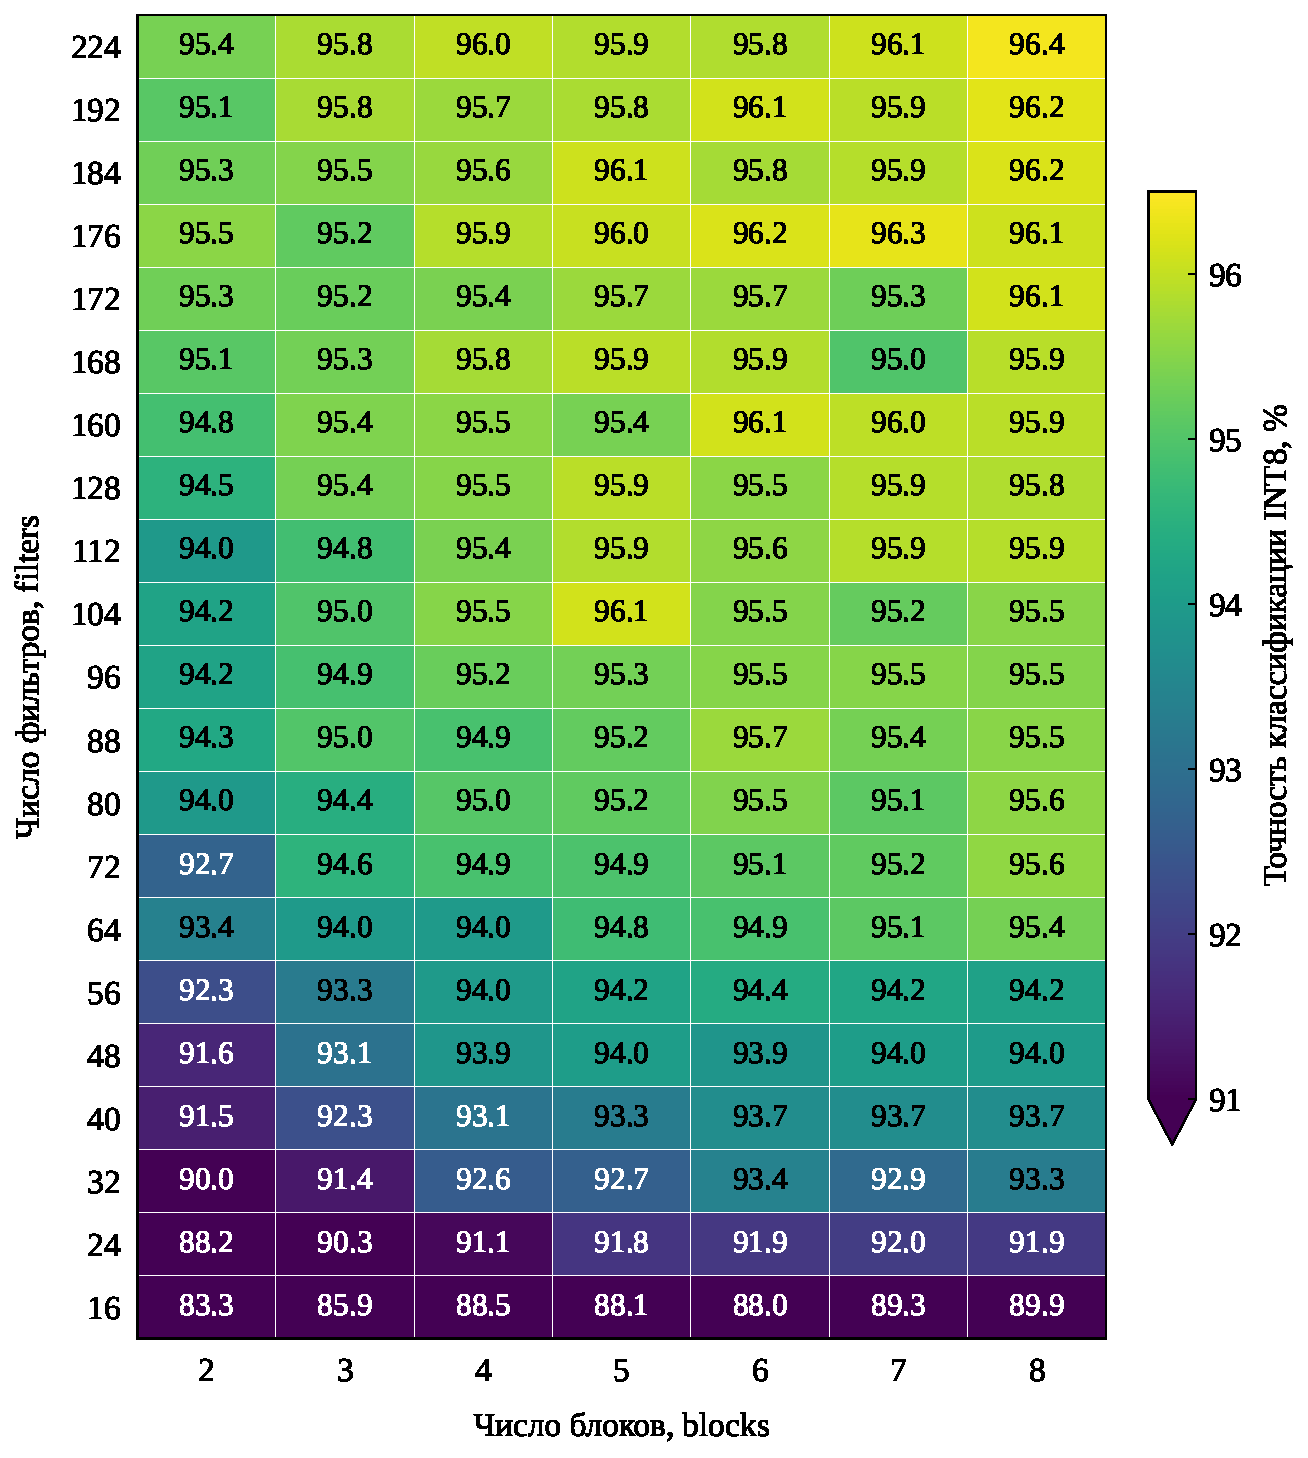
\includegraphics[width=1\textwidth]{assets/diagrams/heatmap_filters_blocks.pdf}
	\caption{Тепловая карта точности INT8-моделей DS-CNN в пространстве гиперпараметров (filters $\times$ blocks)}
	\label{fig:heatmap_filters_blocks}
\end{figure}

Анализ тепловой карты выявляет две закономерности.
\textit{Первая}~--- точность выходит на статистически значимое
плато при $F \geq 80$ и $B \geq 4$, в пределах которого
изменение гиперпараметров не приводит к различиям в точности,
превышающим доверительный интервал Уилсона $\pm 0{,}65$~п.п.
для тестовой выборки $n = 4154$ (формула~\ref{eq:wilson}
раздела~3). \textit{Вторая}~--- для архитектур с малым числом
фильтров ($F < 64$) глубина сети оказывает существенное
влияние на точность, тогда как для $F \geq 80$ зависимость
точности от глубины сглаживается. Содержательная интерпретация
этих наблюдений: при ограниченной ёмкости свёрточных слоёв сеть
выигрывает от дополнительных уровней абстракции; при достаточной
ёмкости дополнительная глубина не даёт значимого выигрыша.

\subsubsection{Парето-граница по размеру модели}

Парето-граница архитектур в координатах
<<точность~$\times$~размер модели INT8>> по 134~обученным
архитектурам и 239~оцениваемым точкам (FP32, PTQ, QAT) приведена
на рис.~\ref{fig:pareto_size_acc}.

\begin{figure}[H]
	\centering
	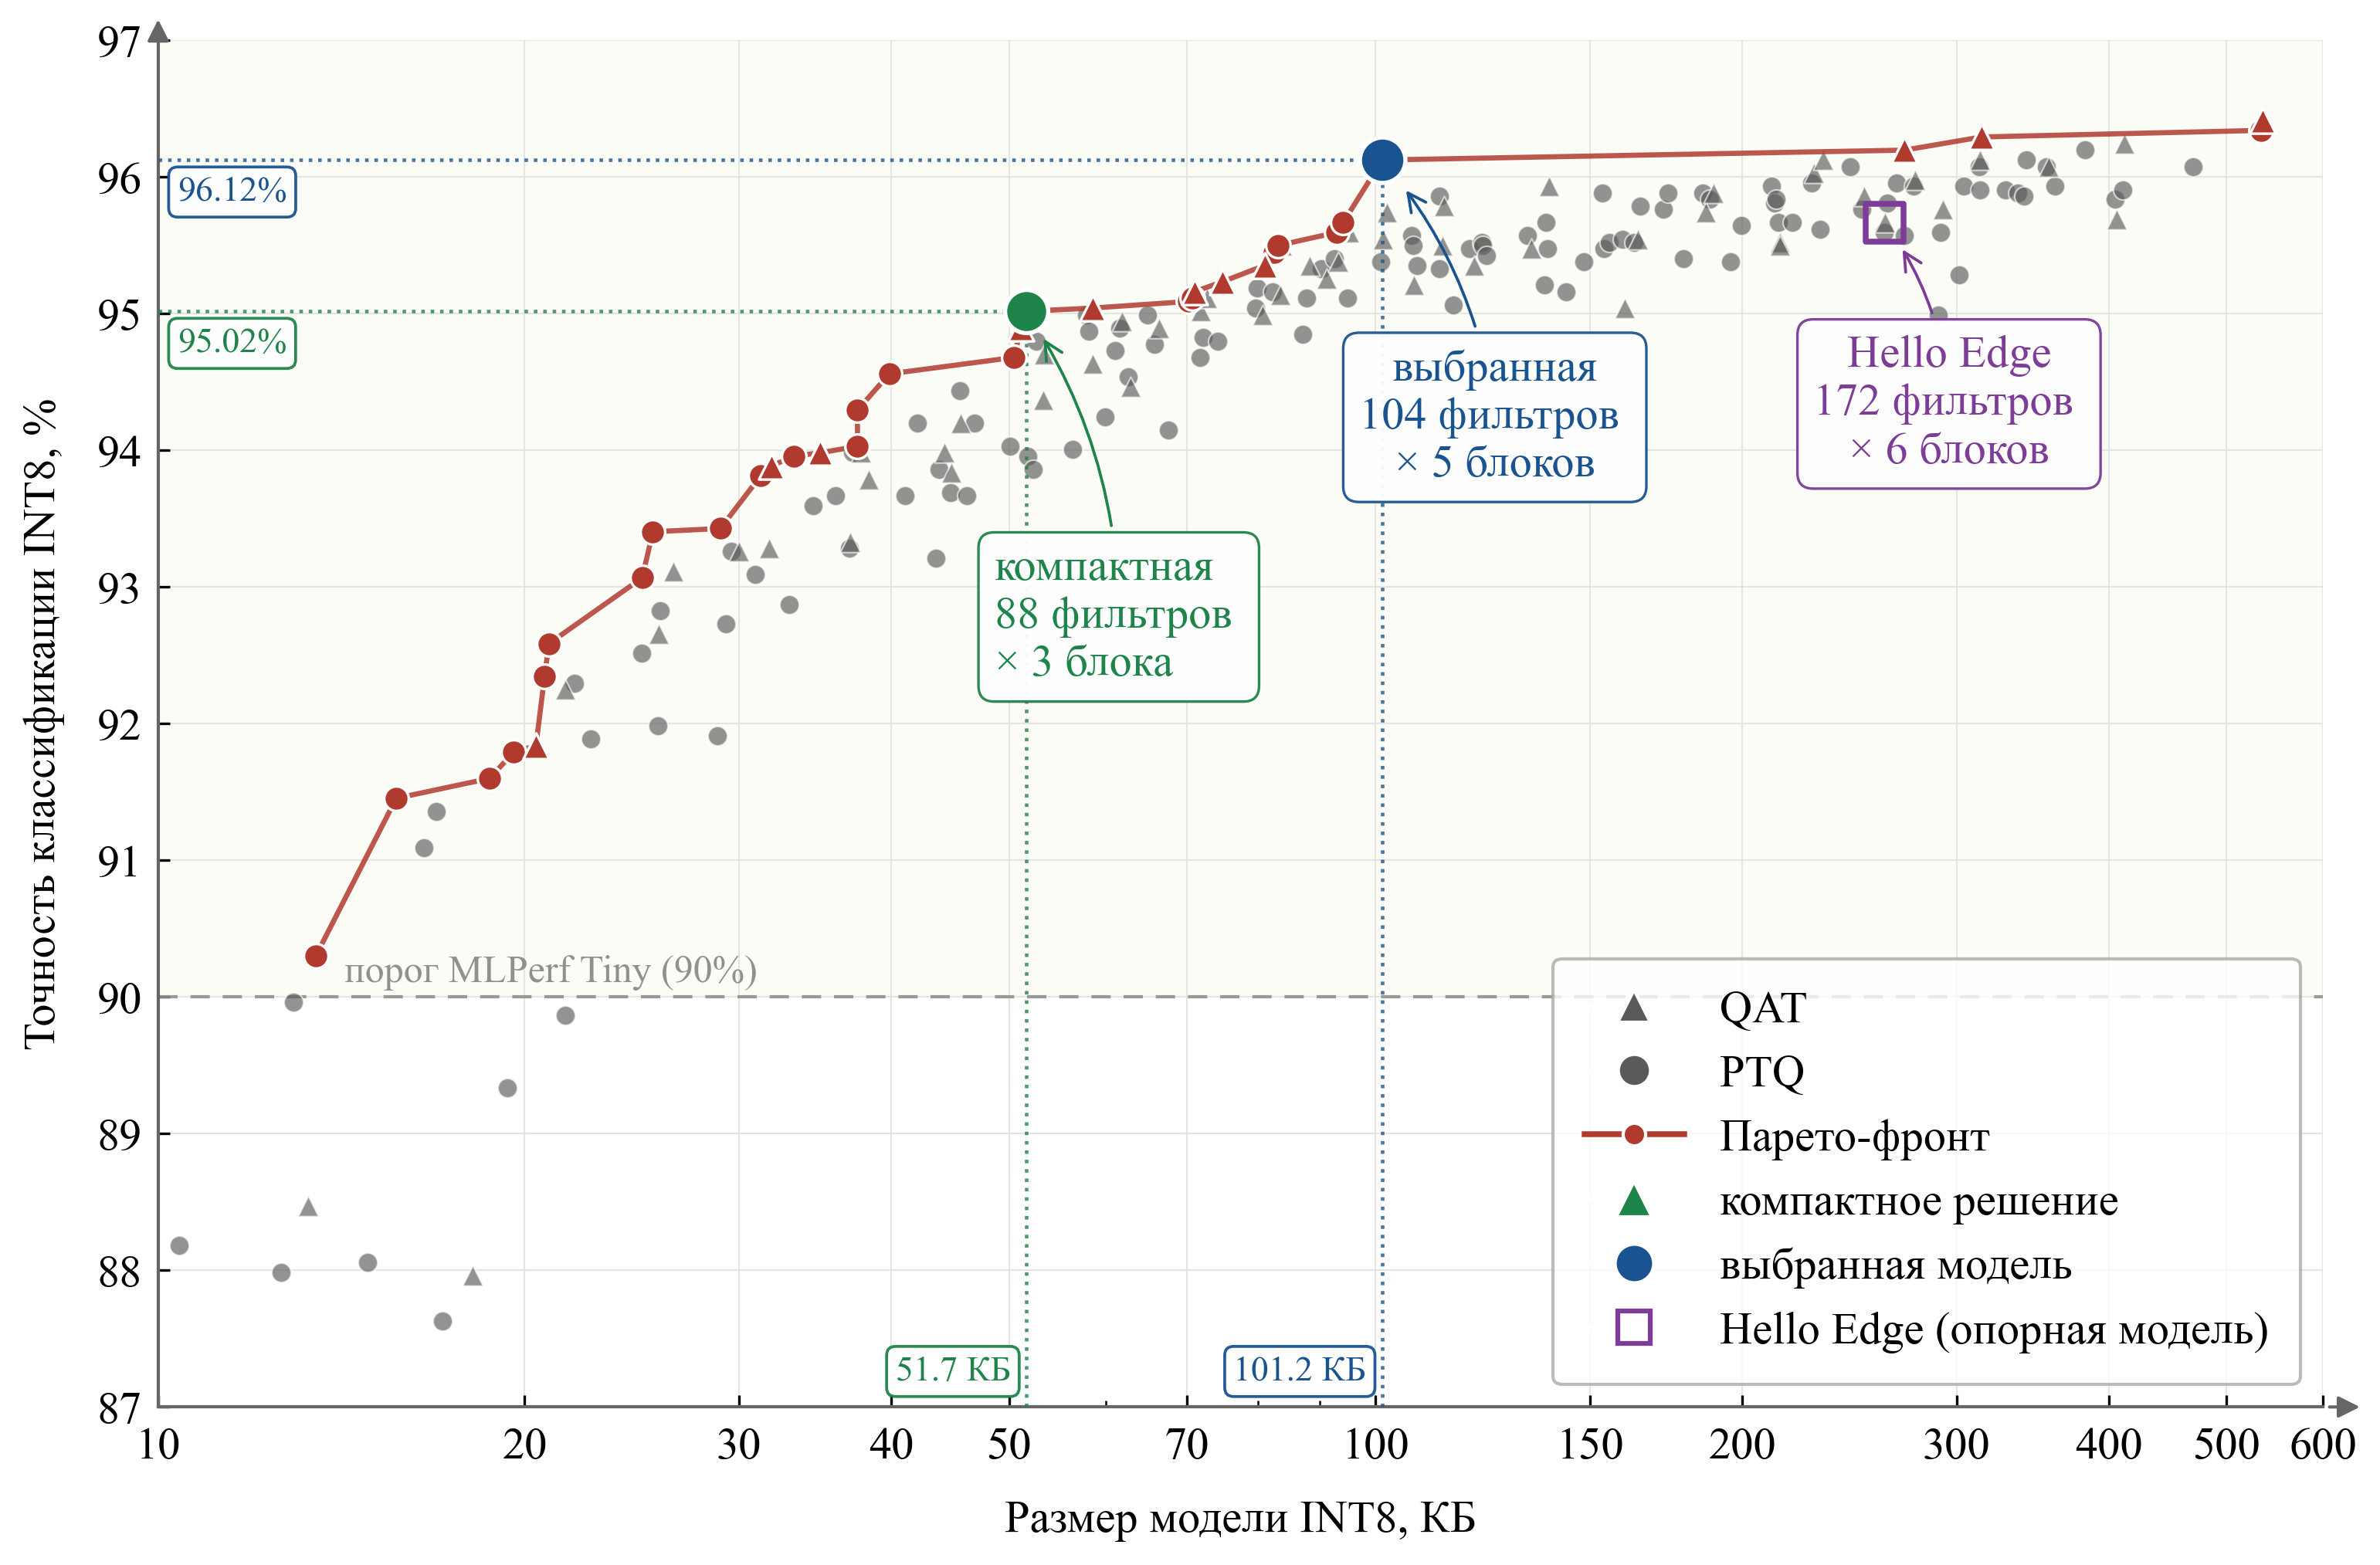
\includegraphics[width=1\textwidth]{assets/plots/pareto_frontier_size_acc.png}
	\caption{Парето-граница архитектур DS-CNN в координатах точность INT8 $\times$ размер модели}
	\label{fig:pareto_size_acc}
\end{figure}

Анализ Парето-границы позволяет выделить четыре характерные
зоны.

\textit{Зона ультракомпактных моделей} ($< 20$~КБ, точность
менее 92\%)~--- архитектуры с предельно малым числом фильтров,
не удовлетворяющие порогу точности 90\% бенчмарка MLPerf
Tiny~\cite{src:5} либо находящиеся на его границе. Применимы
только при крайне строгих ограничениях на флеш-память.

\textit{Зона компромисса} (20--80~КБ, точность 92--95\%)~---
архитектуры с умеренным числом фильтров, обеспечивающие
быстрый рост точности при увеличении размера модели.
Содержательный градиент Парето-границы в этой зоне~--- порядка
0,1~п.п. точности на каждый дополнительный килобайт размера
модели.

\textit{Зона оптимума} (80--110~КБ, точность 95--96\%)~---
архитектуры, для которых точность достигает значений в пределах
1~п.п. от верхней границы исследованного диапазона. Парето-knee
данной зоны находится в области моделей с $F \approx 100$,
$B = 5$, и обоснование выбора финальной модели именно из этой
зоны проводится в подразделе~4.4.

\textit{Зона насыщения} (более 110~КБ)~--- архитектуры, в
которых дальнейшее увеличение размера не приводит к
статистически значимому росту точности. Эталонная конфигурация
Hello Edge DS-CNN-M~\cite{src:1} ($F = 172$, $B = 6$,
размер $\approx 260$~КБ) располагается в этой зоне и не
является Парето-оптимальной для исследованной задачи на
платформе ESP32-S3.

\subsection{Сравнение методов квантизации PTQ и QAT}
\label{subsec:ptq_vs_qat}

В соответствии с задачей~3 введения проведено сравнение методов
квантизации PTQ и QAT. Сопоставление выполнено на двух уровнях
обобщения. На первом уровне~--- детальное сравнение для четырёх
представительных архитектур, перекрывающих весь диапазон
исследованных размеров: компактная $f24\_b5$ (20~КБ), средняя
$f72\_b4$ (51~КБ), эталонная Hello Edge $f176\_b6$ (272~КБ) и
выбранная финальная $f104\_b5$ (101~КБ). На втором уровне~---
агрегированный статистический анализ парных различий точности
$\Delta = \mathrm{acc_{QAT}} - \mathrm{acc_{PTQ}}$ по всем
63~архитектурам, для которых проведены оба метода. Результаты
обоих уровней сравнения представлены на рис.~\ref{fig:ptq_vs_qat}.

\begin{figure}[H]
	\centering
	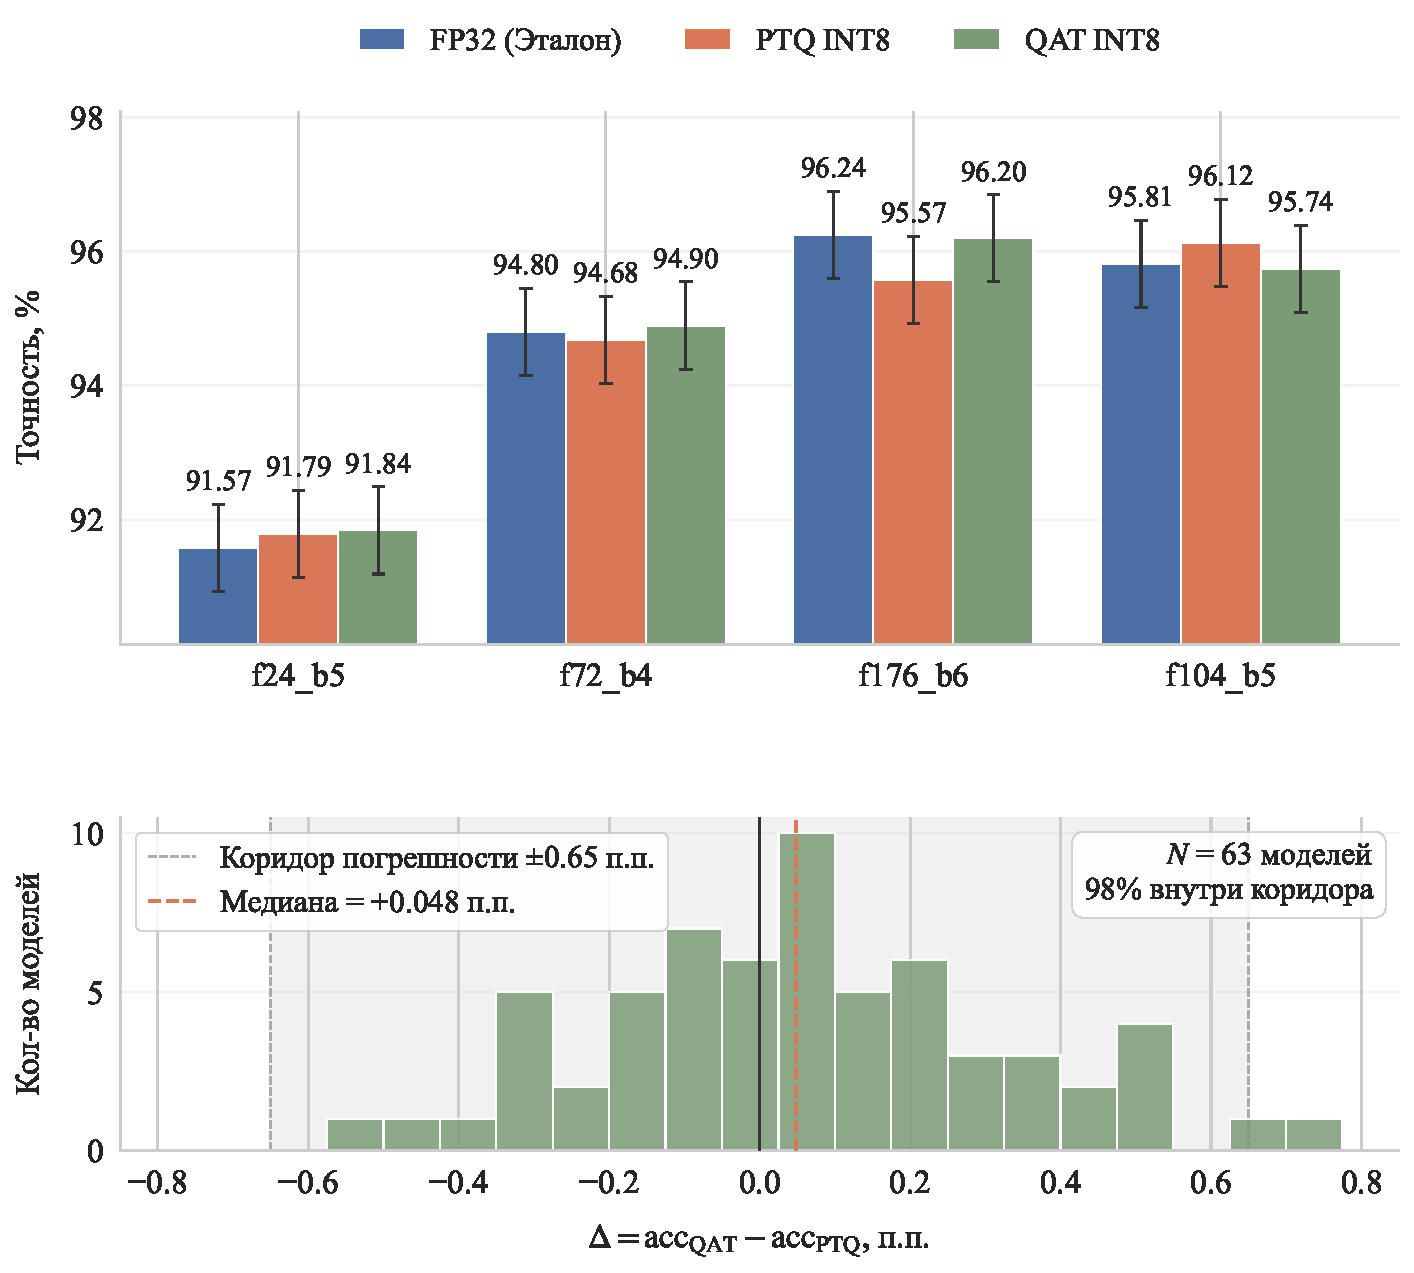
\includegraphics[width=1\textwidth]{assets/diagrams/ptq_vs_qat.pdf}
	\caption{Сравнение методов квантизации PTQ и QAT. Сверху: точность FP32, PTQ INT8 и QAT INT8 для четырёх представительных архитектур с доверительными интервалами Уилсона $\pm 0{,}65$~п.п. Снизу: распределение парных различий $\Delta = \mathrm{acc_{QAT}} - \mathrm{acc_{PTQ}}$ по 63~архитектурам с обоими методами квантизации; серой полосой обозначен коридор статистической погрешности}
	\label{fig:ptq_vs_qat}
\end{figure}

Из приведённого сравнения следуют три наблюдения.

\textit{Первое.} На всех четырёх представительных архитектурах
различия в точности между методами PTQ и QAT не превышают
0,67~п.п. (максимальное различие 0,63~п.п. для $f176\_b6$:
95,57\% PTQ против 96,20\% QAT) и в большинстве случаев
существенно меньше: для $f24\_b5$ различие составляет 0,05~п.п.,
для $f72\_b4$~--- 0,22~п.п., для $f104\_b5$~--- 0,38~п.п. Все
различия лежат в пределах либо непосредственно у границы
доверительного интервала Уилсона ($\pm 0{,}65$~п.п.) и не
являются статистически значимыми.

\textit{Второе.} Агрегированная статистика по 63~парам PTQ/QAT
подтверждает наблюдение первого уровня: 98\% парных различий
$\Delta$ лежат внутри коридора $\pm 0{,}65$~п.п. при медиане
$+0{,}048$~п.п. Распределение различий симметрично относительно
нуля, что указывает на отсутствие систематического преимущества
одного метода над другим для исследованного класса задач
квантизации DS-CNN до INT8.

\textit{Третье.} В отдельных случаях точность квантизованной
модели превышает точность исходной FP32-модели на величину
порядка 0,3~п.п. (для архитектуры $F=104$, $B=5$~--- 96,12\% PTQ
INT8 против 95,81\% FP32; для $F=176$, $B=6$~--- 96,24\% FP32
против 96,20\% QAT INT8 и 95,57\% PTQ INT8). Подобное
наблюдение объясняется статистическим характером оценки и
согласуется с независимыми результатами Сёренсена и
др.~\cite{src:31}, где для аналогичной архитектуры на
платформе Cortex-M4 также отмечались случаи точности
INT8-моделей не ниже FP32. Содержательно эффект
интерпретируется как регуляризационное действие квантизации:
округление весов и активаций вносит шум, который для умеренно
переобученной FP32-модели играет роль сглаживающего
фактора~\cite{src:3}.

\textit{Вывод по задаче~3 введения.} Применительно к задаче
квантизации DS-CNN до INT8 на платформе ESP32-S3 методы PTQ и
QAT обеспечивают статистически неразличимую точность.
Преимущество PTQ состоит в существенно меньшей вычислительной
стоимости~--- отсутствие цикла дообучения сокращает время
получения квантизованной модели с десятков минут до единиц
секунд при сопоставимой точности. Это делает PTQ предпочтительным
методом при условии достаточности INT8-разрядности для целевой
задачи.

\subsection{Анализ времени инференса на платформе ESP32-S3}

Послойная декомпозиция времени инференса, полученная программным
профилированием через \texttt{esp\_timer\_get\_time()} для
подмножества архитектур разного размера, приведена на
рис.~\ref{fig:layer_decomp_ms} (в абсолютных единицах) и
рис.~\ref{fig:layer_decomp_pct} (в относительных долях).

\begin{figure}[H]
	\centering
	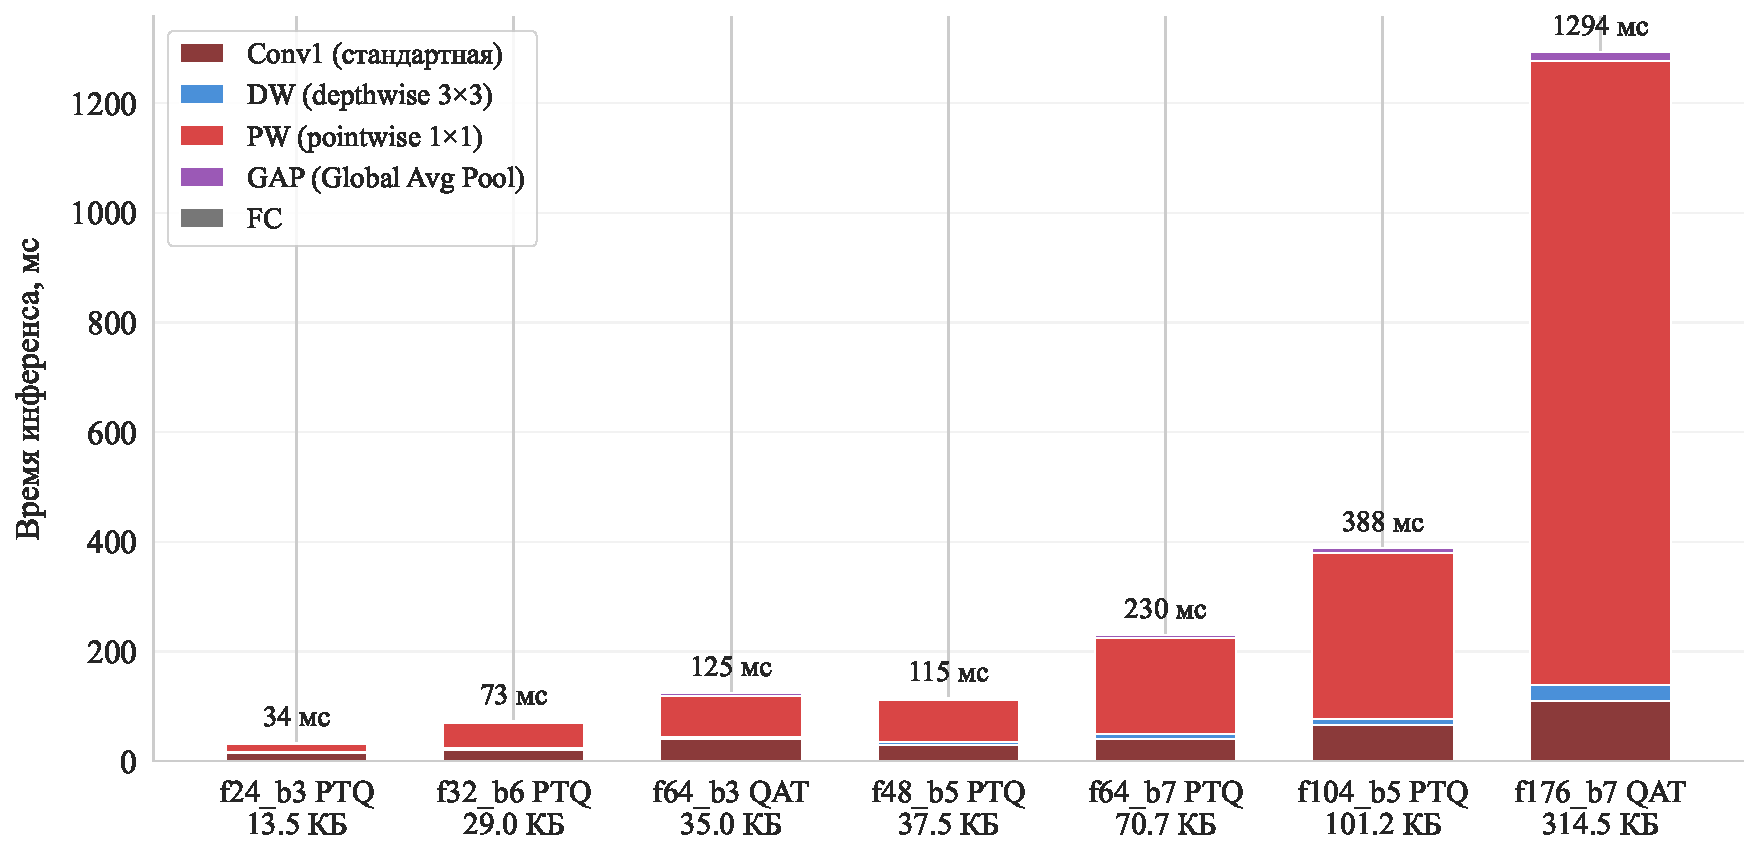
\includegraphics[width=1\textwidth]{assets/diagrams/layer_decomp_A_by_type_ms.pdf}
	\caption{Послойная декомпозиция времени инференса DS-CNN на ESP32-S3 для архитектур различного размера, абсолютные значения}
	\label{fig:layer_decomp_ms}
\end{figure}

\begin{figure}[H]
	\centering
	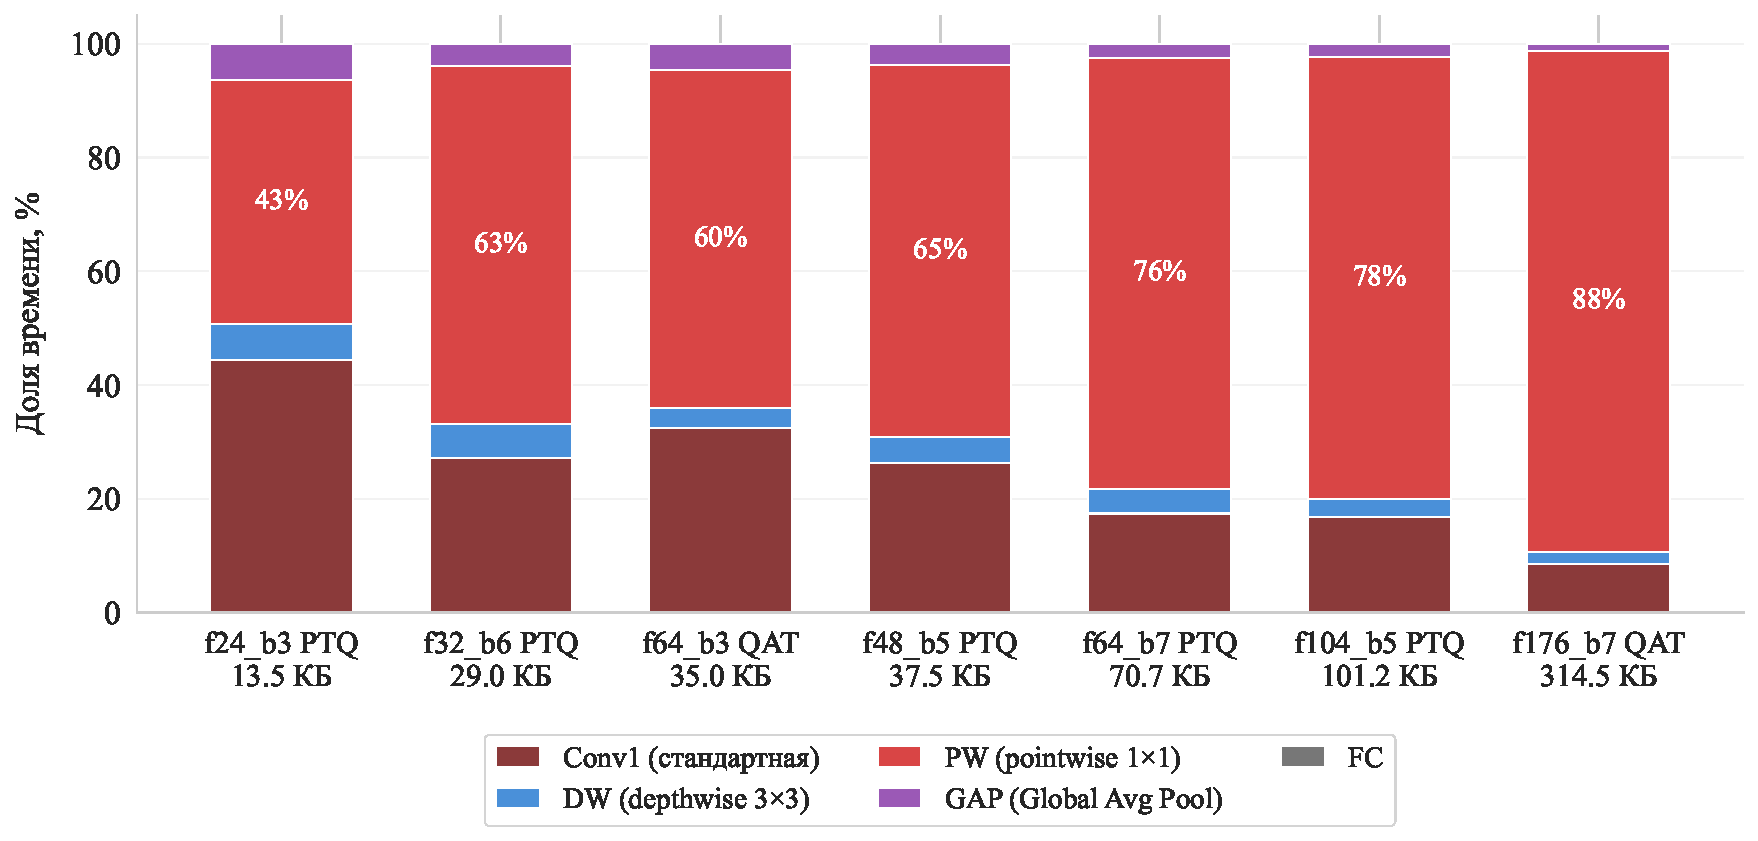
\includegraphics[width=1\textwidth]{assets/diagrams/layer_decomp_A_by_type_pct.pdf}
	\caption{Послойная декомпозиция времени инференса DS-CNN на ESP32-S3 для архитектур различного размера, относительные доли}
	\label{fig:layer_decomp_pct}
\end{figure}

Из приведённой декомпозиции следуют три инженерных вывода.

\textit{Первый.} На всех исследованных архитектурах
доминирующий вклад в время инференса вносят
pointwise-свёртки~--- от примерно 50\% общего времени для
компактных архитектур ($F < 48$) до более 85\% для архитектур с
$F > 128$. Стандартная свёртка первого слоя
(\texttt{stem\_conv}), depthwise-свёртки и финальные операции
(\texttt{Mean}, \texttt{FullyConnected}) в сумме составляют от
четверти до половины времени инференса для компактных моделей и
менее одной шестой для крупных.

\textit{Второй.} С ростом числа фильтров $F$ время выполнения
pointwise-свёрток растёт сверхлинейно (фактор $\sim F^2$,
поскольку pointwise-свёртка содержит $F \times F$ умножений на
выходной пиксель), тогда как остальные операции масштабируются
линейно или сублинейно. Это объясняет наблюдаемую квадратичную
зависимость полного времени инференса от числа фильтров и
полностью согласуется с положением финальной модели $f104\_b5$
в области умеренных $F$, обеспечивающей баланс между точностью
и временем инференса.

\textit{Третий.} Подтверждение использования аппаратного
SIMD-ускорения для pointwise-свёрток получено инструментальным
контролем: внутри \texttt{conv.cc} библиотеки ESP-NN
зафиксирована активация оптимизированного <<fast path>> кода для
всех протестированных конфигураций (число каналов кратно 8).
Несмотря на это, доминирование pointwise-свёрток сохраняется,
что указывает на ограничение, накладываемое самим объёмом
вычислений, а не эффективностью их аппаратного ускорения.

\textit{Практическое следствие.} Оптимизация
энергопотребления нейросетевого инференса на платформе общего
назначения требует прежде всего сокращения числа фильтров
архитектуры, а не углубления сети либо переноса вычислений на
альтернативные аппаратные ускорители. Этот вывод послужил
дополнительным обоснованием выбора финальной модели с умеренным
числом фильтров $F = 104$ при увеличенной глубине $B = 5$
относительно компромисса <<глубже~--- уже>>.

\subsection{Выбор финальной модели по Парето-критерию энергия~$\times$~точность}

Размер модели характеризует архитектуру в отрыве от целевой
платформы. Для финального выбора модели, развёртываемой на
ESP32-S3, основным критерием служит энергия одного нейросетевого
инференса, рассчитываемая по формуле~\eqref{eq:energy_inf}
раздела~3.

\subsubsection{Методика расчёта энергии инференса}

Энергия одного нейросетевого инференса определяется как
интеграл мгновенной мощности по интервалу состояния
\texttt{INFERENCE} цикла каскадной обработки:
\begin{equation}
	E_{\text{инф}} = \int_{t_0}^{t_1} U(t) \cdot I(t) \, dt,
	\label{eq:energy_inf_subsec}
\end{equation}
где $U(t)$ и $I(t)$~--- мгновенные значения напряжения и тока
шины питания микроконтроллера, измеренные монитором мощности
INA228~\cite{src:16} с периодом дискретизации, согласованным с
программными метками состояний; $t_0$ и $t_1$~--- моменты
входа и выхода из состояния \texttt{INFERENCE} соответственно.
Численное интегрирование выполняется методом трапеций по
дискретным отсчётам $(U_k, I_k, t_k)$, что компенсирует
изменение мгновенного тока в пределах состояния и даёт более
точную оценку, чем произведение средних значений.

Для подавления случайной составляющей измерения каждый цикл
каскадной обработки выполняется на лабораторном стенде
троекратно подряд; в качестве оценки энергии инференса принято
среднее арифметическое по трём реализациям, в качестве оценки
погрешности~--- выборочное стандартное отклонение.

\subsubsection{Энергия инференса по подмножеству Парето-границы}

Для подмножества архитектур Парето-границы по размеру модели
(рис.~\ref{fig:pareto_size_acc}) проведены прямые измерения
энергии инференса по формуле~\eqref{eq:energy_inf_subsec}.
Дополнительно в выборку включены архитектуры с шестью
depthwise-separable блоками ($B = 6$) различной ширины
($F \in \{64, 96, 128, 160, 172, 176\}$), позволяющие
охарактеризовать поведение системы в диапазоне размеров модели
от 100 до 270~КБ. Результаты сведены в
табл.~\ref{tab:energy_inf} и графически представлены на
рис.~\ref{fig:pareto_energy_acc}.

\newcolumntype{L}[1]{>{\microtypesetup{activate=true}\RaggedRight\arraybackslash}p{#1}}
\newcolumntype{C}[1]{>{\microtypesetup{activate=true}\Centering\arraybackslash}p{#1}}

\begin{longtable}{|L{2.2cm}|C{2cm}|C{1.6cm}|C{1.5cm}|C{1.4cm}|C{2.6cm}|C{2.1cm}|}
	\caption{Энергетические характеристики архитектур подмножества Парето-границы}
	\label{tab:energy_inf} \\
	\hline
	\textbf{Арх-ра} & \textbf{Метод квантиз.} & \textbf{Размер, КБ} & \textbf{Время, мс} & \textbf{Ток, мА} & \textbf{Энергия, мДж} & \textbf{Точность, \%} \\
	\hline
	\endfirsthead
	\multicolumn{7}{r}{Продолжение таблицы \thetable} \\[6pt]
	\hline
	\textbf{Арх-ра} & \textbf{Метод квантиз.} & \textbf{Размер, КБ} & \textbf{Время, мс} & \textbf{Ток, мА} & \textbf{Энергия, мДж} & \textbf{Точность, \%} \\
	\hline
	\endhead
	\hline
	\endfoot
	f24\_b5  & QAT & 20.4  & 120  & 81.2 & 39.78 $\pm$ 0.41   & 91.84  \\ \hline
	f24\_b3  & PTQ & 13.5  & 120  & 81.5 & 40.09 $\pm$ 1.01   & 90.30  \\ \hline
	f40\_b2  & PTQ & 15.7  & 120  & 82.1 & 40.50 $\pm$ 1.67   & 91.45  \\ \hline
	f32\_b4  & PTQ & 20.9  & 120  & 82.1 & 40.87 $\pm$ 0.88   & 92.59  \\ \hline
	f32\_b6  & PTQ & 29.0  & 140  & 82.6 & 46.57 $\pm$ 11.71  & 93.43  \\ \hline
	f48\_b3  & PTQ & 25.0  & 139  & 83.3 & 47.81 $\pm$ 11.59  & 93.07  \\ \hline
	f48\_b4  & QAT & 31.9  & 160  & 84.3 & 54.91 $\pm$ 10.28  & 93.89  \\ \hline
	f64\_b2  & PTQ & 25.5  & 180  & 82.8 & 60.76 $\pm$ 1.85   & 93.40  \\ \hline
	f48\_b5  & PTQ & 37.5  & 180  & 83.5 & 62.04 $\pm$ 0.50   & 94.03  \\ \hline
	f64\_b3  & QAT & 35.0  & 200  & 82.8 & 66.74 $\pm$ 11.50  & 93.98  \\ \hline
	f72\_b3  & PTQ & 39.9  & 220  & 83.5 & 74.02 $\pm$ 11.75  & 94.56  \\ \hline
	f72\_b4  & QAT & 51.1  & 240  & 83.0 & 82.16 $\pm$ 0.18   & 94.90  \\ \hline
	f88\_b3  & PTQ & 51.7  & 280  & 83.1 & 96.02 $\pm$ 12.43  & 95.02  \\ \hline
	f64\_b7  & PTQ & 70.7  & 300  & 83.1 & 102.01 $\pm$ 1.62  & 95.11  \\ \hline
	f80\_b5  & QAT & 71.0  & 340  & 84.2 & 115.27 $\pm$ 11.08 & 95.16  \\ \hline
	f88\_b6  & PTQ & 94.0  & 417  & 83.3 & 142.64 $\pm$ 8.92  & 95.67  \\ \hline
	f104\_b5 & PTQ & 101.2 & 440  & 83.2 & 149.64 $\pm$ 9.52  & 96.12  \\ \hline
	f176\_b7 & QAT & 314.5 & 1347 & 82.9 & 451.22 $\pm$ 7.58  & 96.29  \\
	\hline
\end{longtable}


\begin{figure}[H]
	\centering
	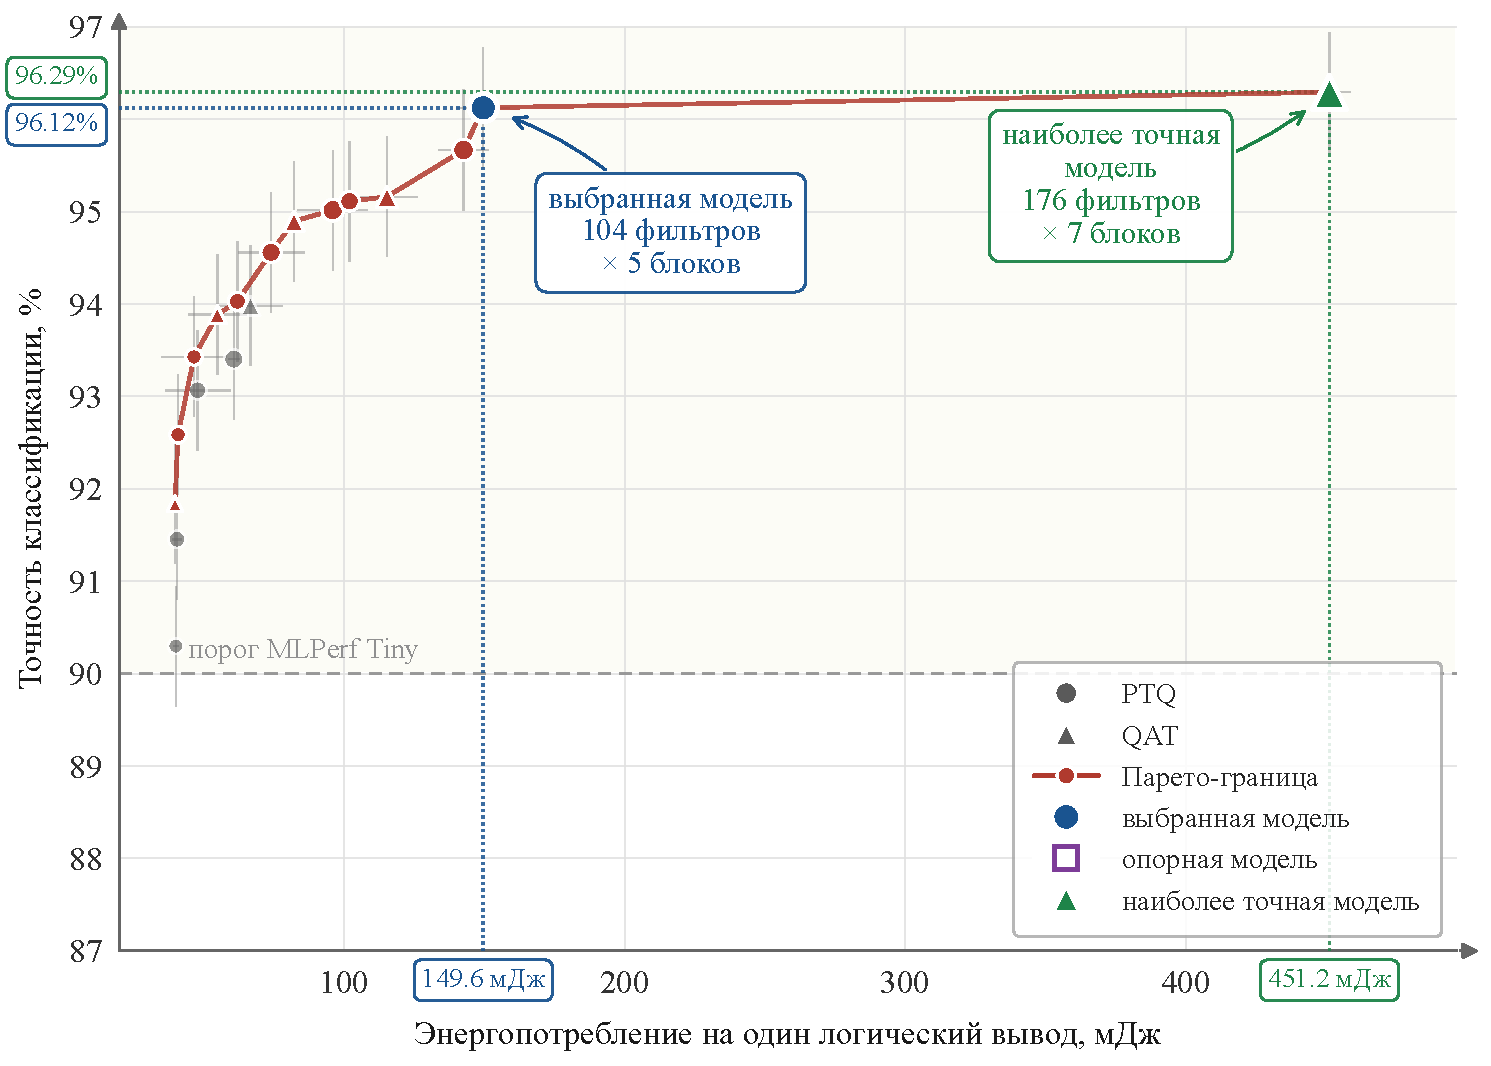
\includegraphics[width=1\textwidth]{assets/plots/pareto_energy_acc.pdf}
	\caption{Парето-граница архитектур DS-CNN в координатах точность классификации~$\times$~энергия одного нейросетевого инференса на платформе ESP32-S3. Серыми маркерами показаны архитектуры, доминируемые по совокупности двух критериев; красной линией соединены архитектуры Парето-границы. Подсвечены выбранная финальная модель $f104\_b5$ (синий) и архитектура с максимальной достижимой точностью в исследованном диапазоне $f176\_b7$ (зелёный)}
	\label{fig:pareto_energy_acc}
\end{figure}

Полученный график иллюстрирует характерную форму границы
Парето в задачах оптимизации нейросетевых архитектур: резкий
прирост точности в области малых значений энергии (от~25 до
100~мДж) сменяется протяжённым участком насыщения, на котором
дальнейшее увеличение вычислительных затрат сопровождается
прибавкой в точности классификации, не превышающей единиц
десятых процентного пункта. Точка излома границы Парето
локализуется в окрестности 150~мДж на инференс, что
соответствует выбранной финальной модели $f104\_b5$.

\subsubsection{Обоснование выбора финальной модели}

Из множества архитектур, удовлетворяющих жёстким критериям
(точность~$\geq 90\%$ из требования MLPerf Tiny~\cite{src:5};
размер модели в пределах внутреннего SRAM платформы для
совместимости с SIMD-ускорением библиотеки ESP-NN; время
инференса в пределах разумной интерактивной задержки), в
качестве финальной модели для развёртывания выбрана архитектура
DS-CNN с $F = 104$, $B = 5$, квантизованная методом PTQ
(далее~--- \texttt{f104\_b5} PTQ).

Обоснование выбора по совокупности критериев:

\begin{itemize}
	\item \textit{Положение в точке излома границы Парето.}
	      Выбранная модель располагается на верхне-левой
	      огибающей графика рис.~\ref{fig:pareto_energy_acc} в
	      точке излома, после которой граница переходит в
	      режим насыщения по точности. Энергия одного
	      инференса составляет 149,6~мДж~--- в 3~раза меньше
	      по сравнению с архитектурой максимальной точности
	      $f176\_b7$ (451,2~мДж) при разнице в точности
	      0,17~п.п. (96,12\% против 96,29\%), не превышающей
	      статистической погрешности оценки.

	\item \textit{Точность классификации $96{,}12\%$}
	      превышает требование MLPerf Tiny ($90\%$) на
	      $6{,}1$~п.п. и отличается от максимальной достижимой
	      в исследованном диапазоне точности $96{,}29\%$
	      (архитектура $f176\_b7$~QAT) на $0{,}17$~п.п., что
	      находится в пределах статистической погрешности
	      оценки точности на тестовой выборке.

	\item \textit{Превосходство над опорной моделью
		      Hello~Edge~\cite{src:1}.} Выбранная архитектура
	      достигает точности, не уступающей опорной модели,
	      при существенно меньшем размере (101~КБ против
	      $\approx 272$~КБ) и меньшей энергии одного инференса.
	      Указанное соотношение демонстрирует, что
	      использованный подход к выбору архитектуры
	      обеспечивает результат, превосходящий типовое
	      решение литературы по совокупности рассматриваемых
	      метрик.

	\item \textit{Метод квантизации PTQ} обеспечивает
	      достижение указанной точности при сжатии модели в
	      3,73~раза относительно FP32-варианта ($377$~КБ FP32
	      $\to$ $101$~КБ INT8) без использования цикла
	      дообучения. Согласно результатам подраздела~\ref{subsec:ptq_vs_qat},
	      различие между PTQ и QAT для рассматриваемой
	      архитектуры не превышает погрешности измерения
	      точности на тестовой выборке, что делает PTQ
	      предпочтительным по совокупности факторов
	      сложности реализации и стоимости разработки.
\end{itemize}

Совокупность приведённых критериев позволяет считать
архитектуру \texttt{f104\_b5} PTQ обоснованным выбором
финальной модели для развёртывания на платформе ESP32-S3 в
составе разрабатываемой системы распознавания ключевых слов.

\subsection{Качество классификации выбранной модели}

\subsubsection{Кривые обучения}

Динамика обучения FP32-варианта выбранной модели~--- кривые
функции потерь и точности классификации на обучающей и
валидационной выборках~--- представлена на
рис.~\ref{fig:training_curves}.

\begin{figure}[H]
	\centering
	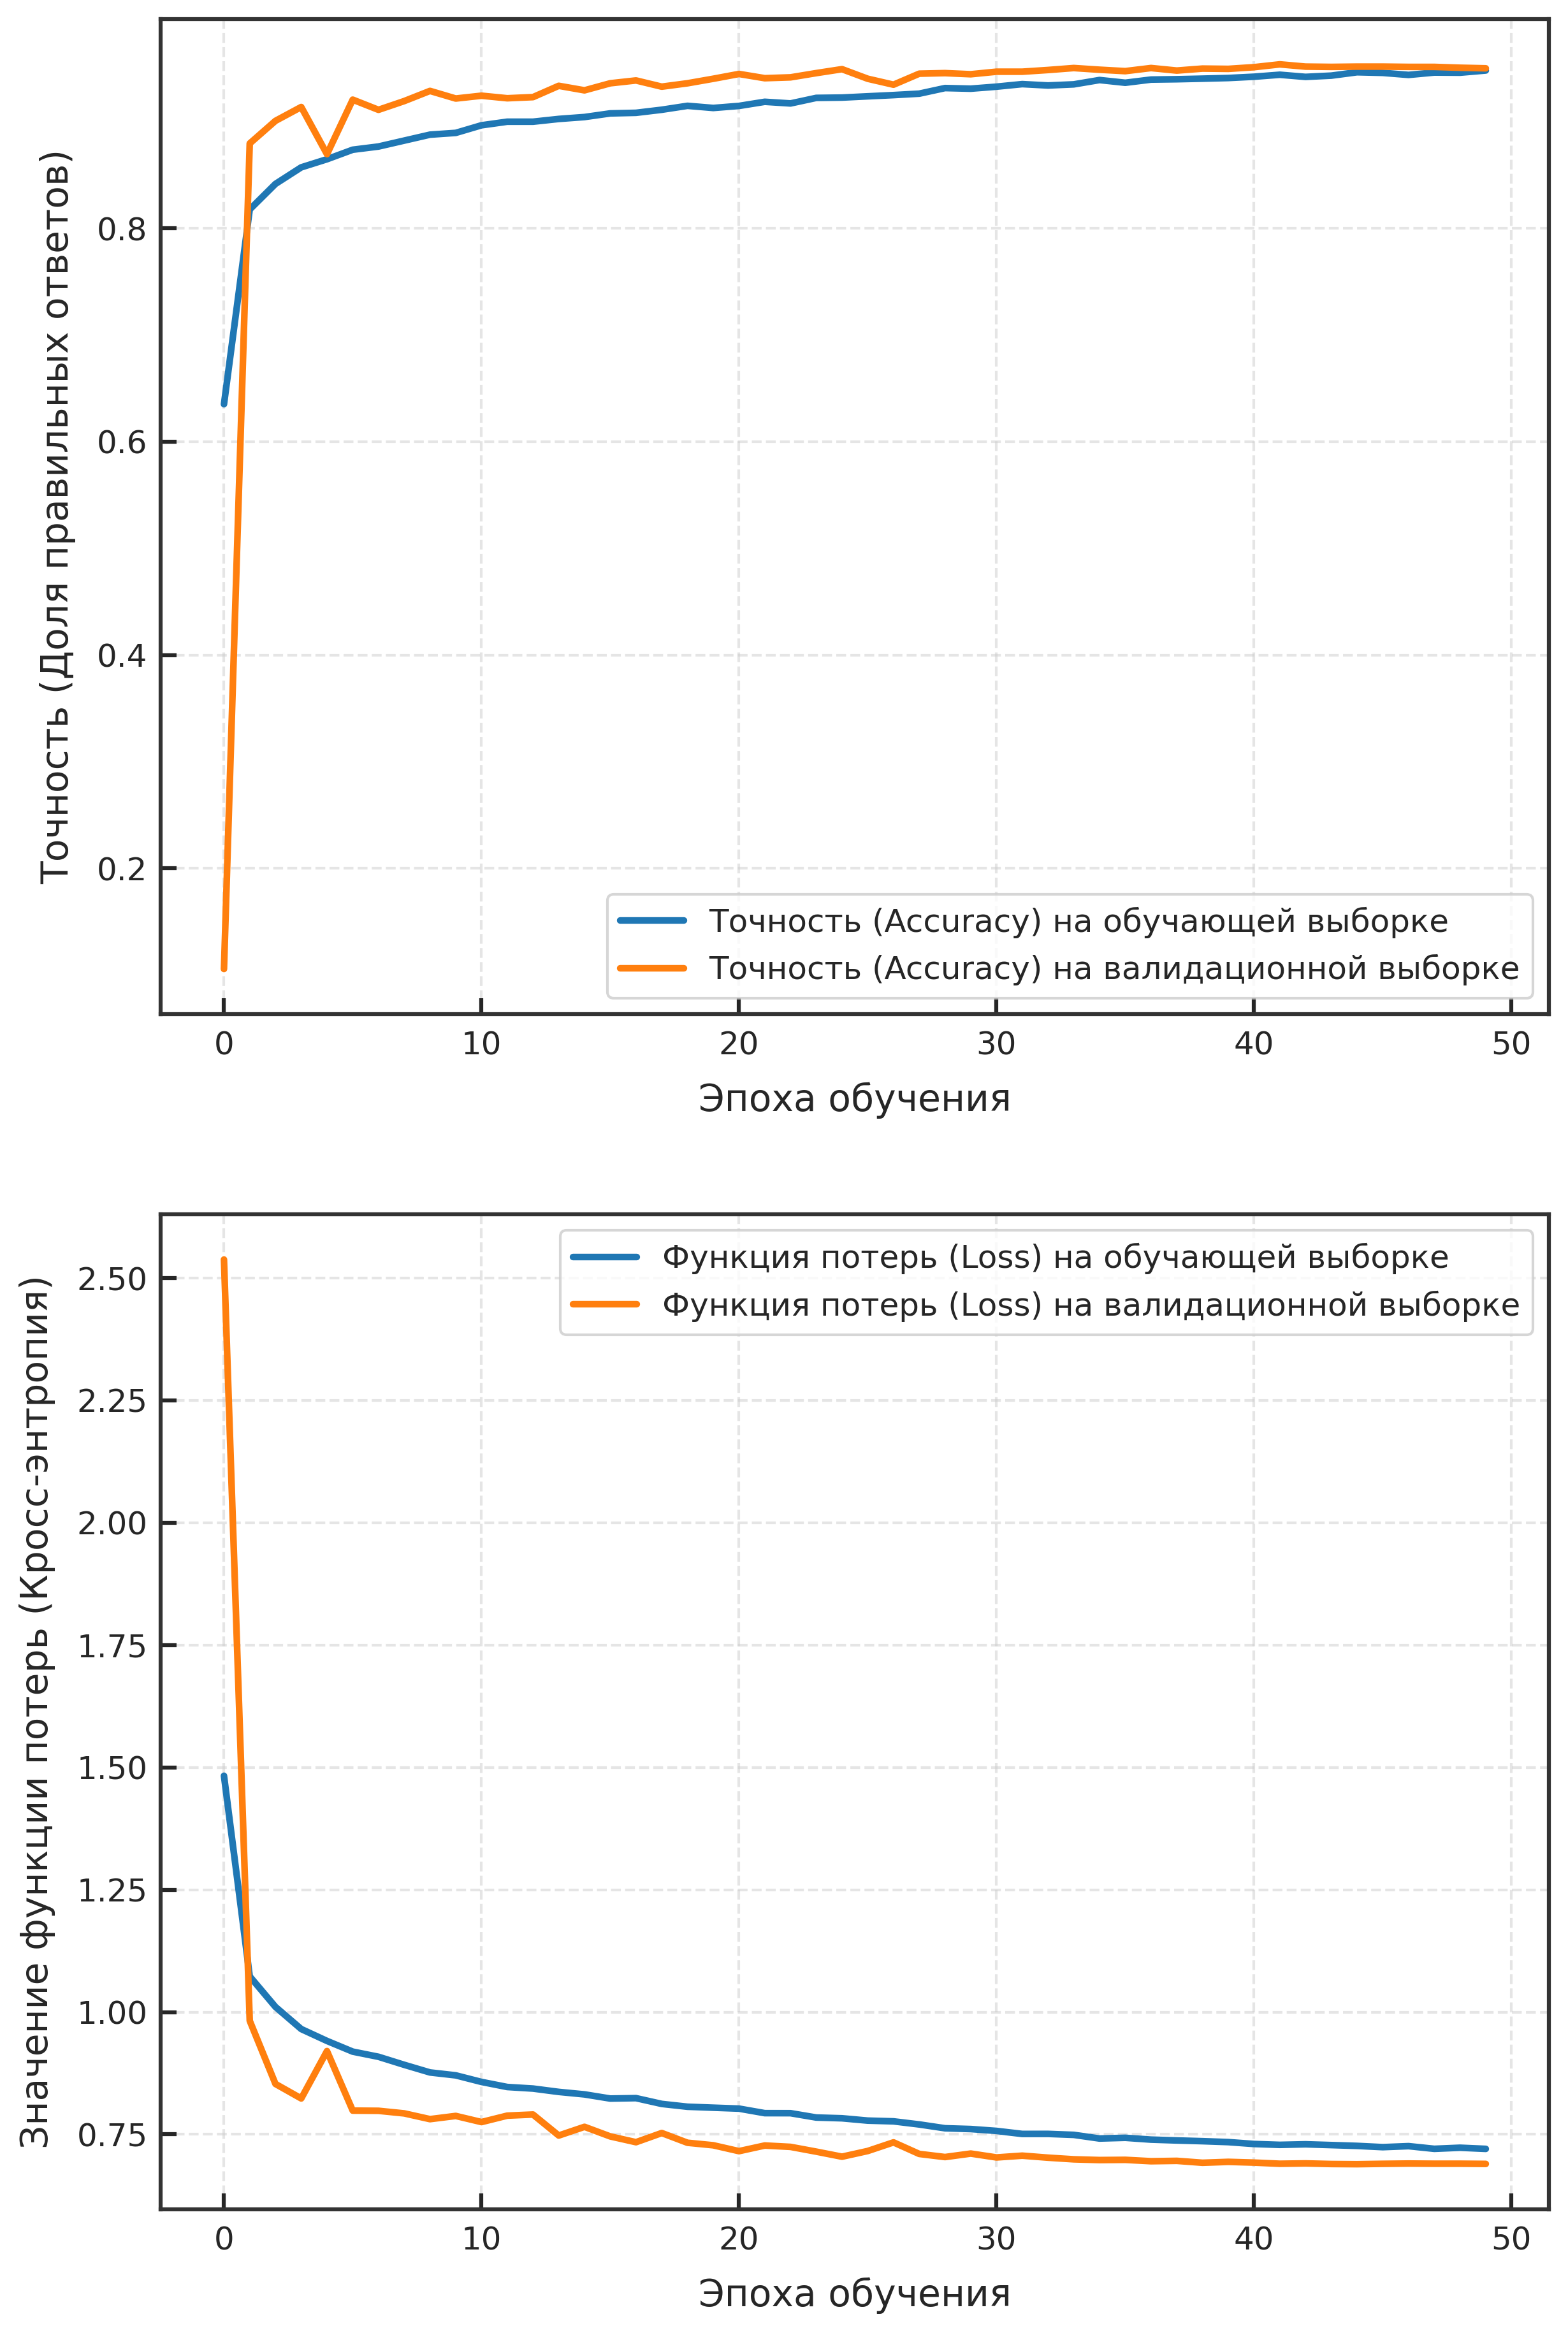
\includegraphics[width=0.65\textwidth]{assets/plots/f104_b5_learning_curves.png}
	\caption{Кривые обучения модели $f104\_b5$ (FP32): функция потерь и точность классификации на обучающей и валидационной выборках по эпохам}
	\label{fig:training_curves}
\end{figure}

Валидационная точность стабилизируется в пределах последних
эпох обучения, разрыв между обучающей и валидационной точностью
сохраняется в пределах нескольких процентных пунктов, что
свидетельствует о сходимости обучения без признаков
существенного переобучения~--- эффект сглаживания меток (label
smoothing) и аугментации данных временны\'{м} сдвигом
обеспечивает необходимую регуляризацию.

\subsubsection{Метрики качества классификации по классам}

Подробные метрики качества классификации квантизованного
варианта PTQ INT8 выбранной модели на тестовой выборке Google
Speech Commands~v2 приведены в
таблице~\ref{tab:classification_metrics}.

\newcolumntype{C}[1]{>{\microtypesetup{activate=true}\centering\arraybackslash}p{#1}}
\begin{longtable}{|C{3.5cm}|C{2.5cm}|C{2.5cm}|C{2.5cm}|C{2.5cm}|}
	\caption{Метрики качества классификации модели $f104\_b5$ PTQ INT8 на тестовой выборке Google Speech Commands~v2}
	\label{tab:classification_metrics}                                                                  \\
	\hline
	\textbf{Класс}        & \textbf{Precision} & \textbf{Recall} & \textbf{F1-score} & \textbf{Support} \\
	\hline
	\endfirsthead
	\hline
	\textbf{Класс}        & \textbf{Precision} & \textbf{Recall} & \textbf{F1-score} & \textbf{Support} \\
	\hline
	\endhead
	\hline
	\endfoot
	yes                   & 0,9647             & 0,9785          & 0,9716            & 419              \\ \hline
	no                    & 0,9429             & 0,9778          & 0,9600            & 405              \\ \hline
	up                    & 0,9543             & 0,9341          & 0,9441            & 425              \\ \hline
	down                  & 0,9348             & 0,9532          & 0,9439            & 406              \\ \hline
	left                  & 0,9780             & 0,9733          & 0,9757            & 412              \\ \hline
	right                 & 0,9949             & 0,9848          & 0,9898            & 396              \\ \hline
	on                    & 0,9642             & 0,9520          & 0,9581            & 396              \\ \hline
	off                   & 0,9500             & 0,9453          & 0,9476            & 402              \\ \hline
	stop                  & 0,9781             & 0,9781          & 0,9781            & 411              \\ \hline
	go                    & 0,9370             & 0,9254          & 0,9312            & 402              \\ \hline
	unknown               & 1,0000             & 1,0000          & 1,0000            & 40               \\ \hline
	silence               & 0,7368             & 0,7000          & 0,7179            & 40               \\ \hline
	\textbf{Macro avg}    & \textbf{0,9446}    & \textbf{0,9419} & \textbf{0,9432}   & 4154             \\ \hline
	\textbf{Weighted avg} & \textbf{0,9581}    & \textbf{0,9581} & \textbf{0,9580}   & 4154             \\
	\hline
\end{longtable}


Поклассовый анализ выявляет следующее.

\textit{Класс silence} демонстрирует ощутимо более низкие
метрики (F1 = 0,72) при минимальном размере выборки данного
класса (40~образцов из 4154). Низкое качество классификации
класса silence объясняется методикой обучения, в которой
образцы тишины генерировались искусственно из фоновых шумов
набора Google Speech Commands; в реальных условиях работы
системы класс silence играет роль фильтра ложных срабатываний
и не критичен для качества основной задачи распознавания
команд.

\textit{Класс unknown} демонстрирует точность 100\%, что
объясняется характером класса: он объединяет все нецелевые
слова из набора и для классификатора представляет более
выраженный паттерн отличия от целевых команд.

\textit{Целевые команды} демонстрируют F1 в диапазоне 0,93--0,99
с macro avg F1 = 0,9432 (по 12~классам) и weighted avg F1 =
0,9580. Минимальные значения F1 наблюдаются на парах
акустически близких слов (\textit{no}/\textit{go},
\textit{on}/\textit{off})~--- ошибки концентрируются именно на
этих парах, что подтверждается анализом матриц ошибок
(рис.~\ref{fig:cm_fp32}--\ref{fig:cm_qat}).

\subsubsection{Матрицы ошибок}

Матрицы ошибок FP32, PTQ INT8 и QAT INT8 вариантов выбранной
модели на тестовой выборке представлены на
рис.~\ref{fig:cm_fp32}--\ref{fig:cm_qat}.

\begin{figure}[H]
	\centering
	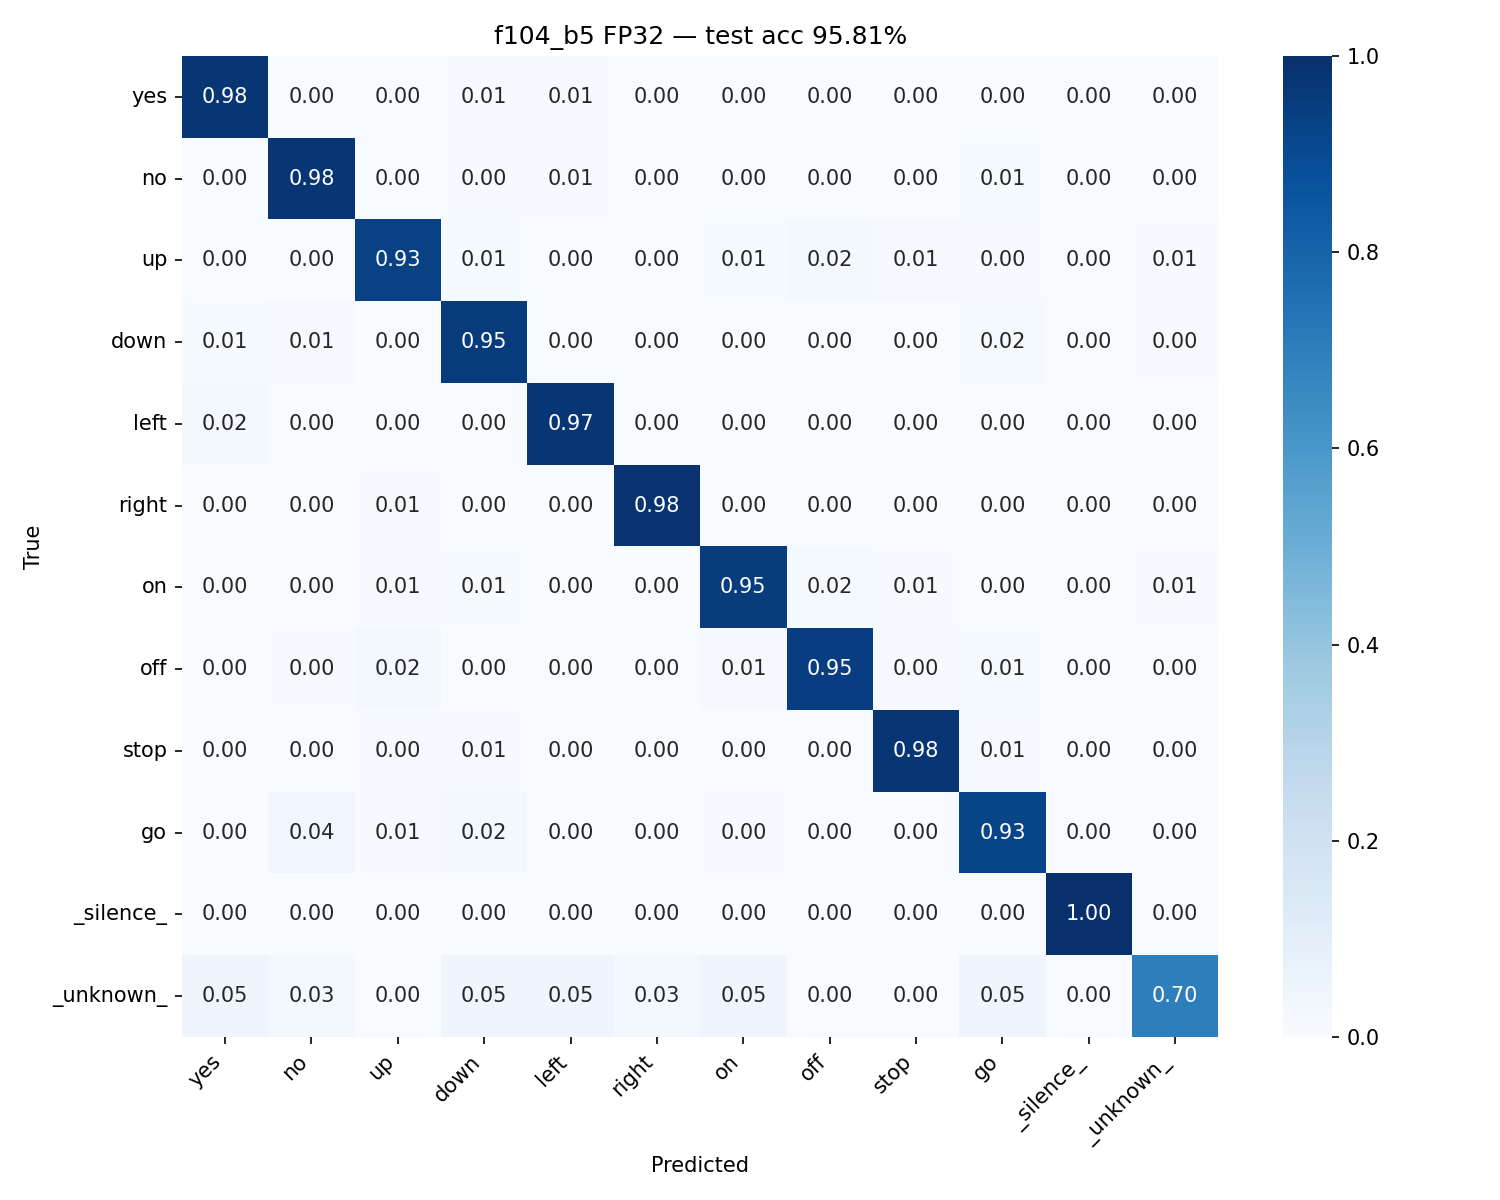
\includegraphics[width=1\textwidth]{assets/diagrams/cm_fp32.png}
	\caption{Матрица ошибок базовой модели $f104\_b5$ (FP32)}
	\label{fig:cm_fp32}
\end{figure}

\begin{figure}[H]
	\centering
	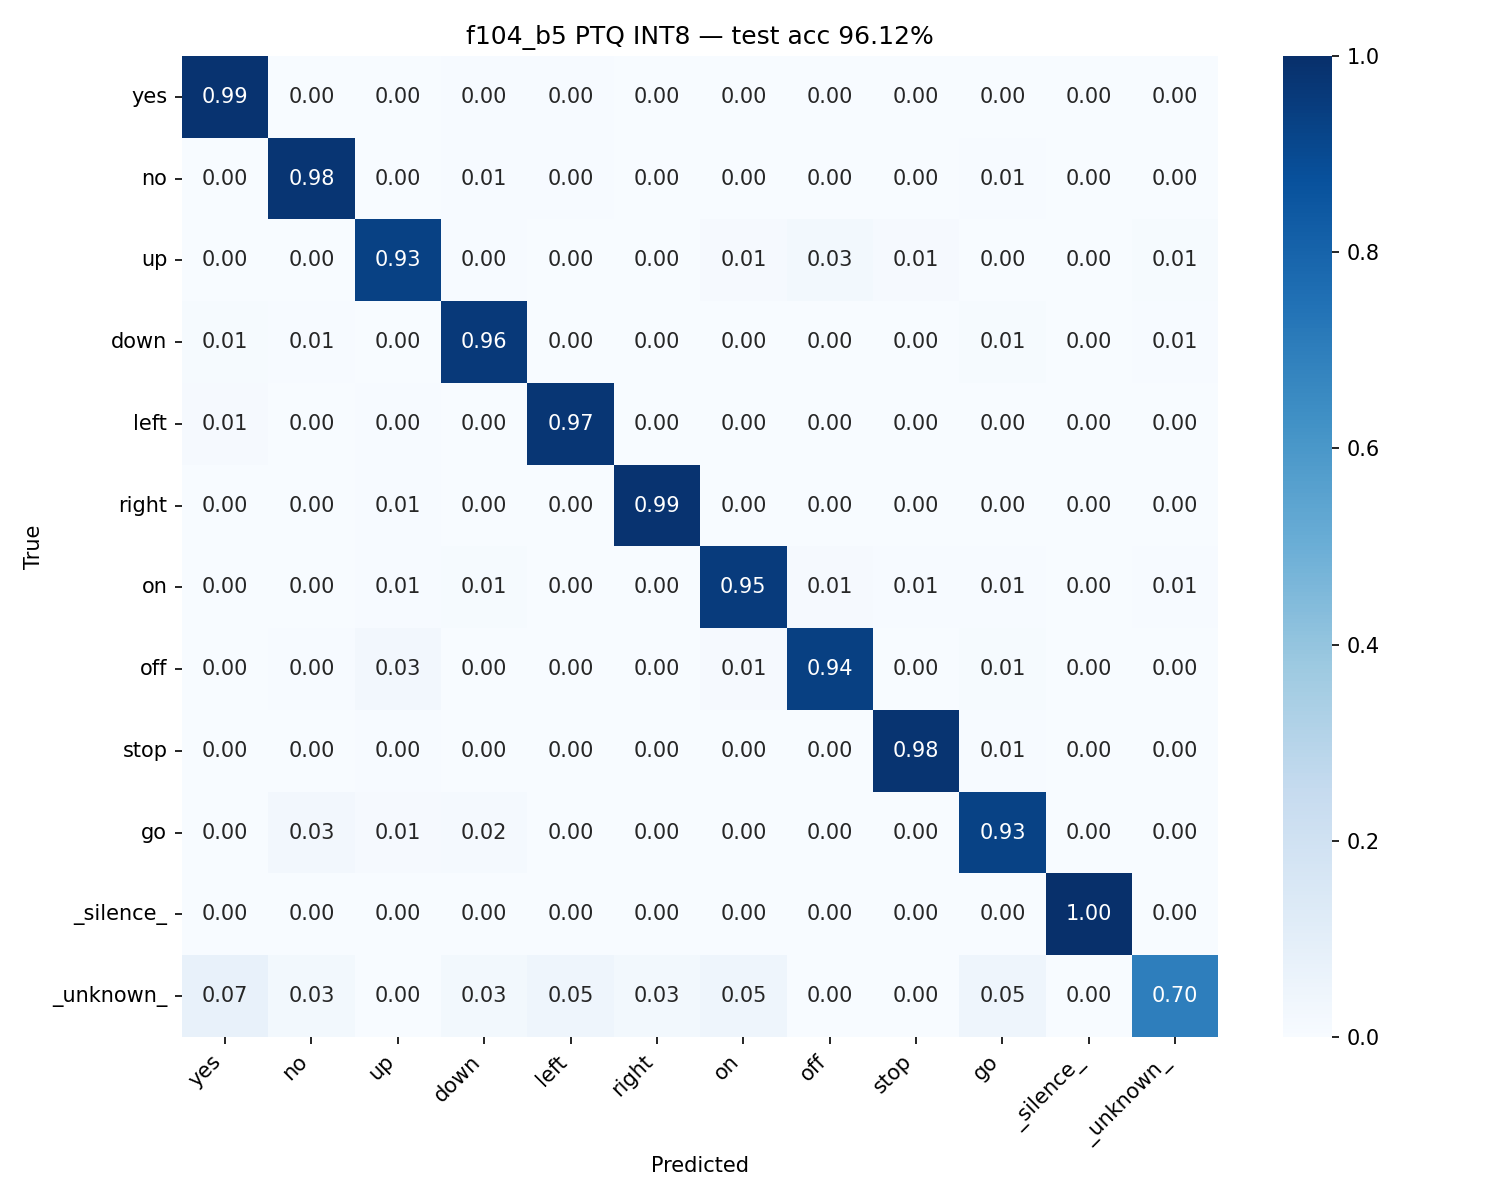
\includegraphics[width=0.85\textwidth]{assets/diagrams/cm_ptq.png}
	\caption{Матрица ошибок квантованной модели $f104\_b5$ (PTQ INT8)}
	\label{fig:cm_ptq}
\end{figure}

\begin{figure}[H]
	\centering
	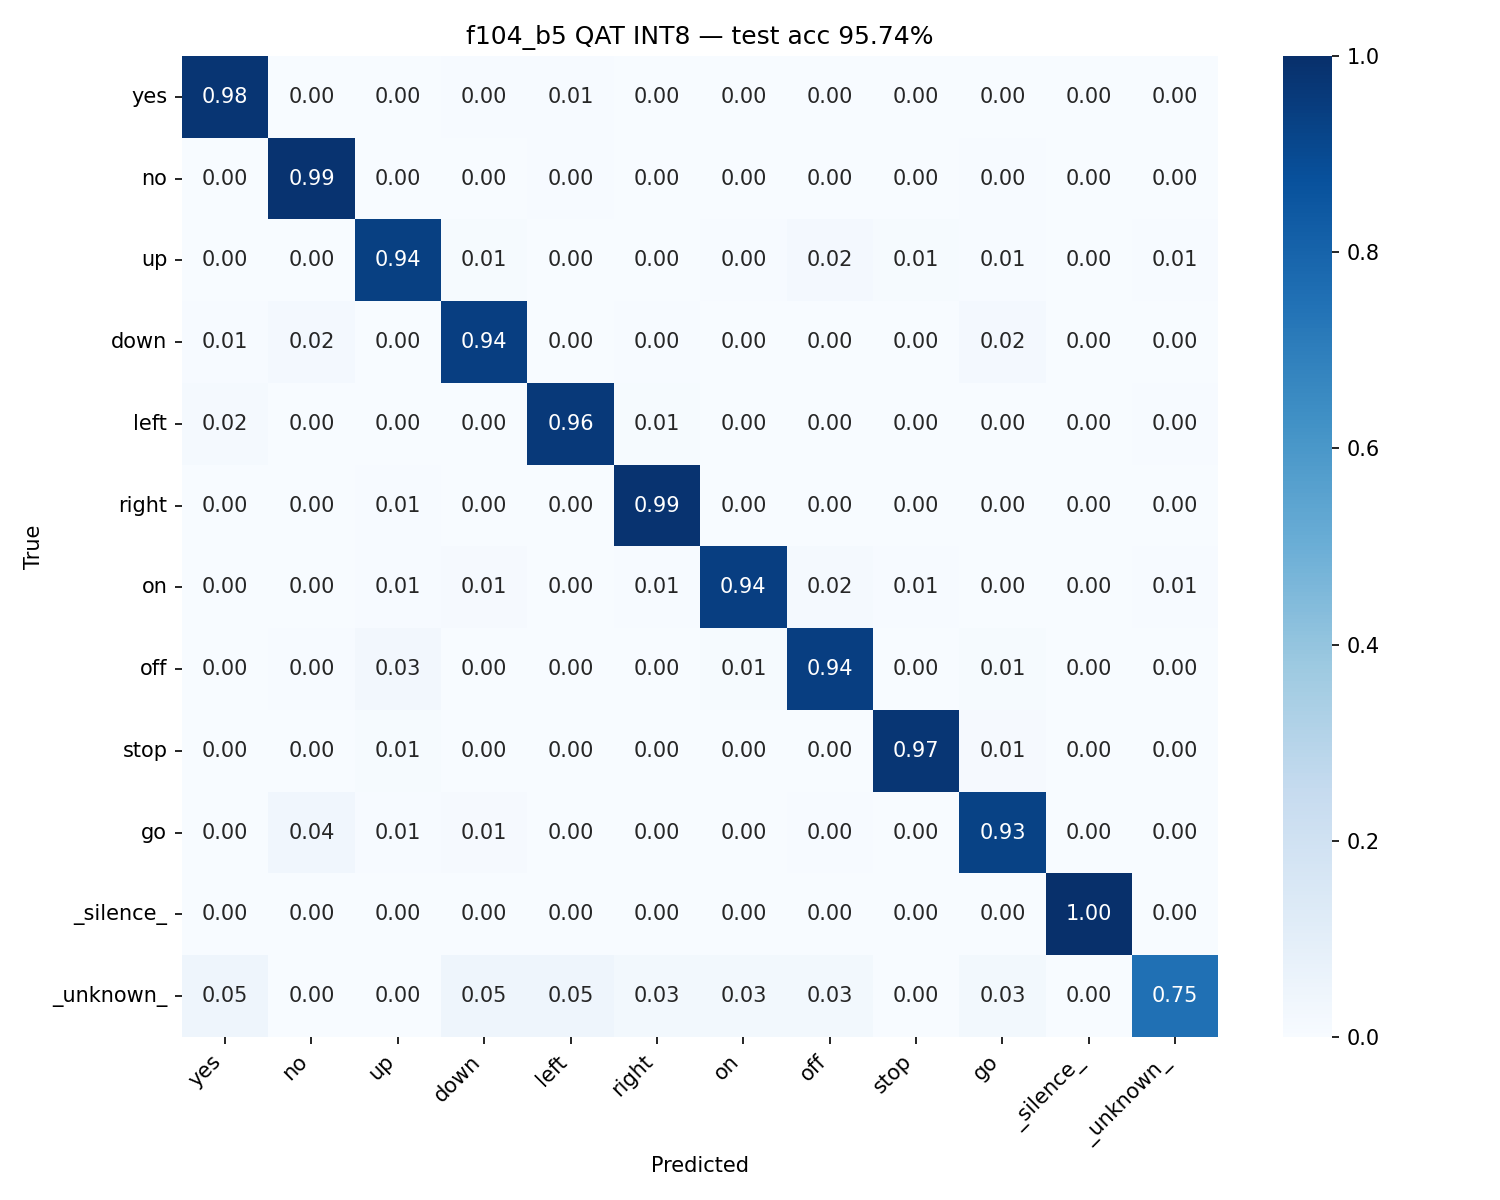
\includegraphics[width=0.85\textwidth]{assets/diagrams/cm_qat.png}
	\caption{Матрица ошибок квантованной модели $f104\_b5$ (QAT INT8)}
	\label{fig:cm_qat}
\end{figure}

Визуальное сравнение матриц подтверждает количественный вывод
подраздела~\ref{subsec:ptq_vs_qat}: структура ошибок
сохраняется при переходе от FP32 к INT8 (как PTQ, так и QAT).
Основная масса ошибок концентрируется в нескольких
внедиагональных ячейках, соответствующих парам акустически
близких слов; квантизация не вносит качественно новых
паттернов ошибок, а лишь равномерно снижает уверенность
классификатора на тех же примерах, на которых модель ошибалась
в FP32-варианте.

При анализе результатов обнаруживается характерный феномен:
точность квантованной модели $f104\_b5$ после применения
процедуры PTQ INT8 (96,12\%) оказалась незначительно выше
исходного варианта FP32 (95,81\%). Различие в 0,31~п.п. не
является статистически значимым и полностью находится в
пределах доверительного интервала Уилсона ($\pm 0{,}65$~п.п.)
для используемого объёма тестовой выборки при $n = 4154$.
Подобное поведение, при котором целочисленная модель показывает
точность на уровне или несколько выше исходной, согласуется с
независимыми результатами Сёренсена и др.~\cite{src:31}.

С содержательной инженерной точки зрения данный эффект
объясняется тем, что квантование весов и активаций до 8-битного
представления вносит контролируемый шум округления, который
действует как форма регуляризации. Для исходной FP32-модели,
обладающей некоторой избыточной ёмкостью, этот сглаживающий
фактор позволяет снизить слабую степень переобучения и
незначительно улучшить обобщающую способность на независимой
тестовой выборке. Подобный регуляризационный эффект
дискретизации весов подробно описан в работе Jacob и
др.~\cite{src:3}.

\subsection{Профиль энергопотребления полного цикла каскадной обработки}

Профиль мгновенного тока, регистрируемый INA228 в течение
полного цикла каскадной обработки от пробуждения по сигналу
EXT1 до возврата в режим глубокого сна, для выбранной модели
$f104\_b5$ PTQ представлен на рис.~\ref{fig:cascade_profile}.
На профиле визуально различимы все состояния конечного
автомата, что подтверждает корректность схемы
GPIO-синхронизации, описанной в подразделе~3.1.

\begin{figure}[H]
	\centering
	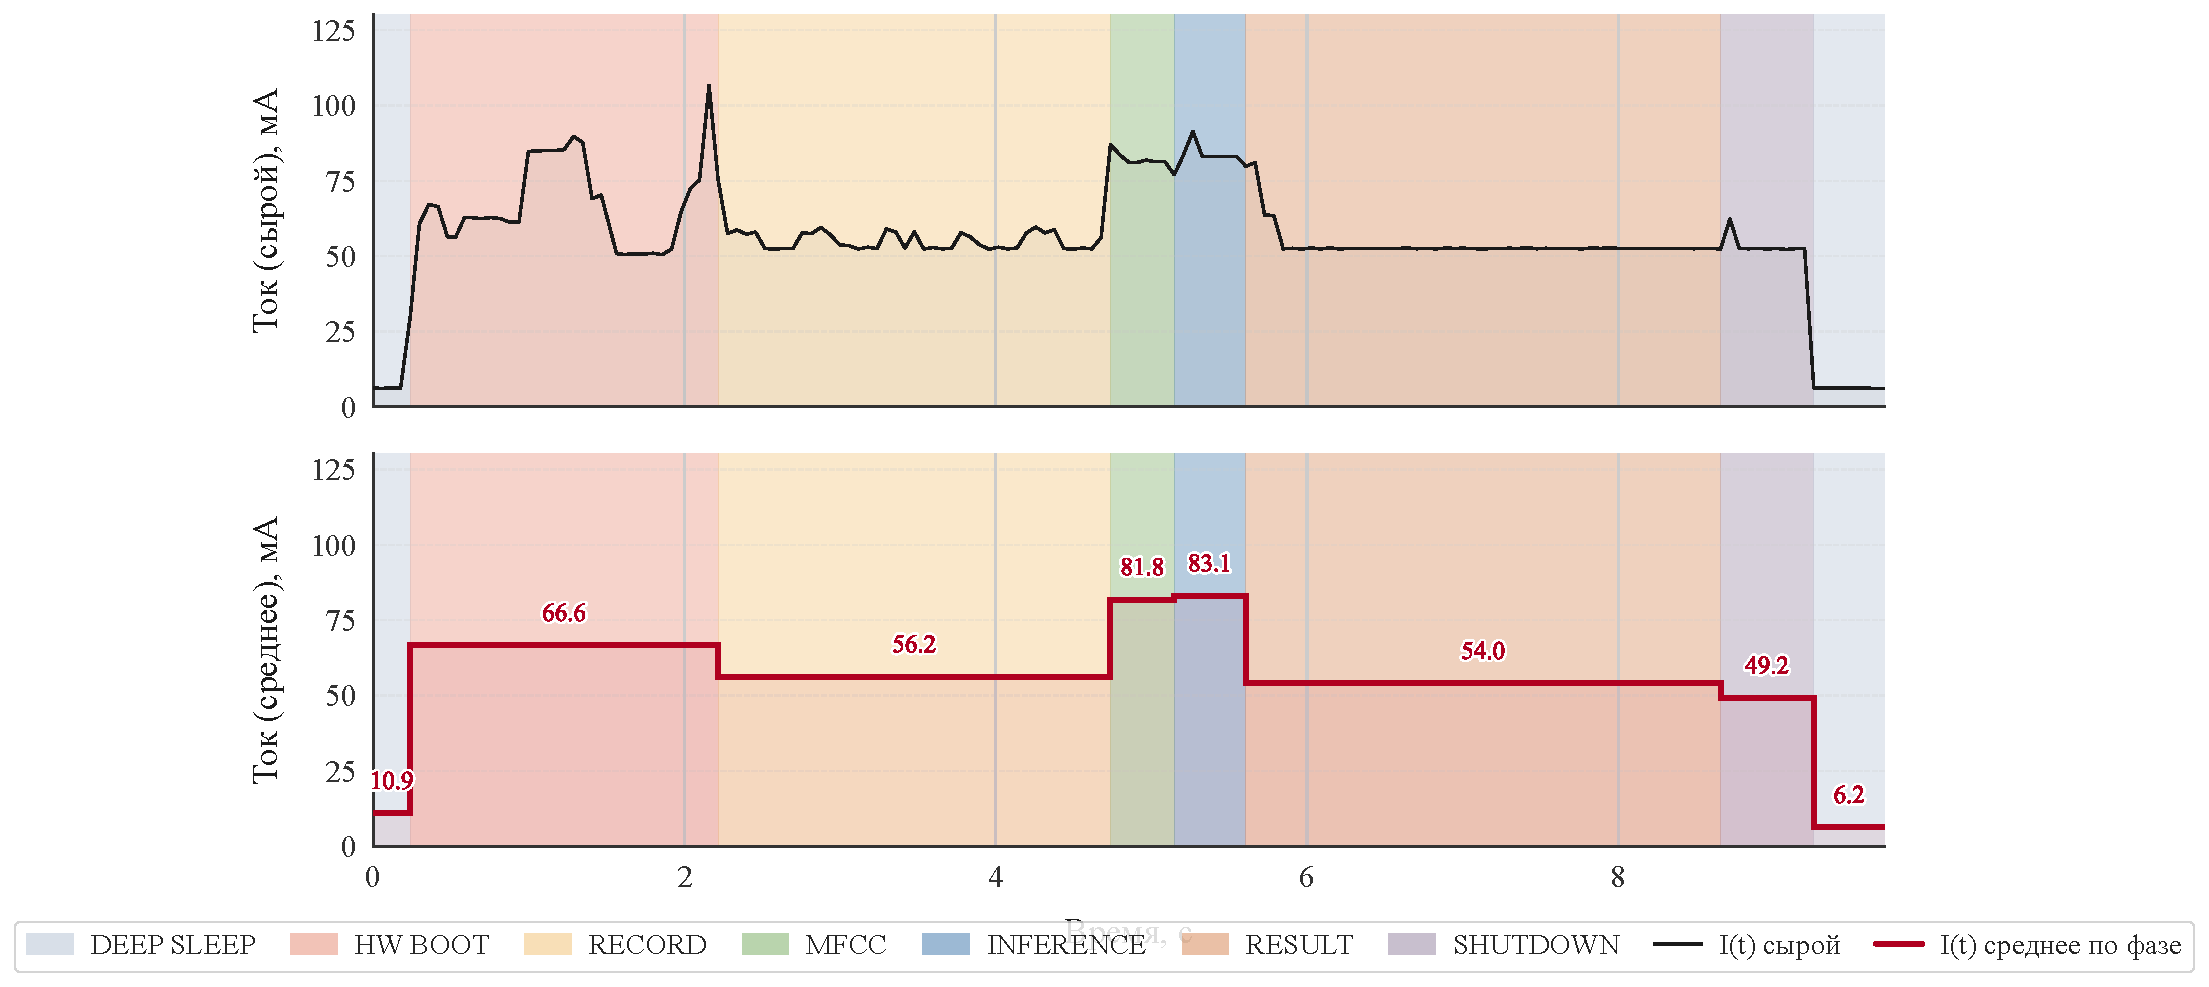
\includegraphics[width=1\textwidth]{assets/diagrams/fig4_6_current_profile.pdf}
	\caption{Профиль мгновенного тока полного цикла каскадной обработки выбранной модели $f104\_b5$ PTQ на платформе ESP32-S3. Сверху: исходный сигнал тока с детальной разметкой состояний FSM. Снизу: усреднённые по состояниям значения тока с численными метками}
	\label{fig:cascade_profile}
\end{figure}

Длительности и средние значения тока на каждом участке,
полученные автоматическим разделением CSV-файла измерений по
биту состояния FSM, сведены в табл.~\ref{tab:fsm_measurements}.

\begin{longtable}{|p{4.5cm}|c|c|}
	\caption{Длительности и средние значения тока на этапах каскадной обработки для модели $f104\_b5$ PTQ}
	\label{tab:fsm_measurements}                                                         \\
	\hline
	\textbf{Этап (состояние FSM)} & \textbf{Длительность, мс} & \textbf{Средний ток, мА} \\
	\hline
	\endfirsthead
	\hline
	\textbf{Этап (состояние FSM)} & \textbf{Длительность, мс} & \textbf{Средний ток, мА} \\
	\hline
	\endhead
	\hline
	\endfoot
	Глубокий сон (DEEP\_SLEEP)    & ---                       & 6,2                      \\ \hline
	Инициализация (HW\_BOOT)      & 1982                      & 66,6                     \\ \hline
	Захват аудио (RECORD)         & 2519                      & 56,2                     \\ \hline
	Извлечение MFCC (MFCC)        & 410                       & 81,8                     \\ \hline
	Инференс DS-CNN (INFERENCE)   & 460                       & 83,1                     \\ \hline
	Завершение (SHUTDOWN)         & 597                       & 49,2                     \\
	\hline
\end{longtable}


\subsection{Декомпозиция энергобюджета цикла}

Энергия, расходуемая на одно полное прохождение каскадного
цикла, вычислена по формуле~\eqref{eq:energy_cycle} численным
интегрированием мгновенной мощности по показаниям INA228.
Декомпозиция энергобюджета по состояниям конечного автомата
приведена в табл.~\ref{tab:energy_decomp} и графически~--- на
рис.~\ref{fig:energy_donut}.

\begin{longtable}{|p{4.5cm}|c|c|c|}
	\caption{Декомпозиция энергопотребления одного цикла каскадной обработки для модели $f104\_b5$ PTQ}
	\label{tab:energy_decomp}                                                                              \\
	\hline
	\textbf{Этап}                 & \textbf{Длит., мс} & \textbf{Энергия, мДж} & \textbf{Доля бюджета, \%} \\
	\hline
	\endfirsthead
	\hline
	\textbf{Этап}                 & \textbf{Длит., мс} & \textbf{Энергия, мДж} & \textbf{Доля бюджета, \%} \\
	\hline
	\endhead
	\hline
	\endfoot
	Инициализация (HW\_BOOT)      & 1982               & 532,57                & 34,9                      \\ \hline
	Захват аудио (RECORD)         & 2519               & 569,74                & 37,4                      \\ \hline
	Извлечение MFCC (MFCC)        & 410                & 137,19                & 9,0                       \\ \hline
	Инференс DS-CNN (INFERENCE)   & 460                & 155,65                & 10,2                      \\ \hline
	Завершение (SHUTDOWN)         & 597                & 130,21                & 8,5                       \\ \hline
	\textbf{Итого за цикл}        & \textbf{5968}      & \textbf{1525,4}       & \textbf{100,0}            \\
	\hline
\end{longtable}


\begin{figure}[H]
	\centering
	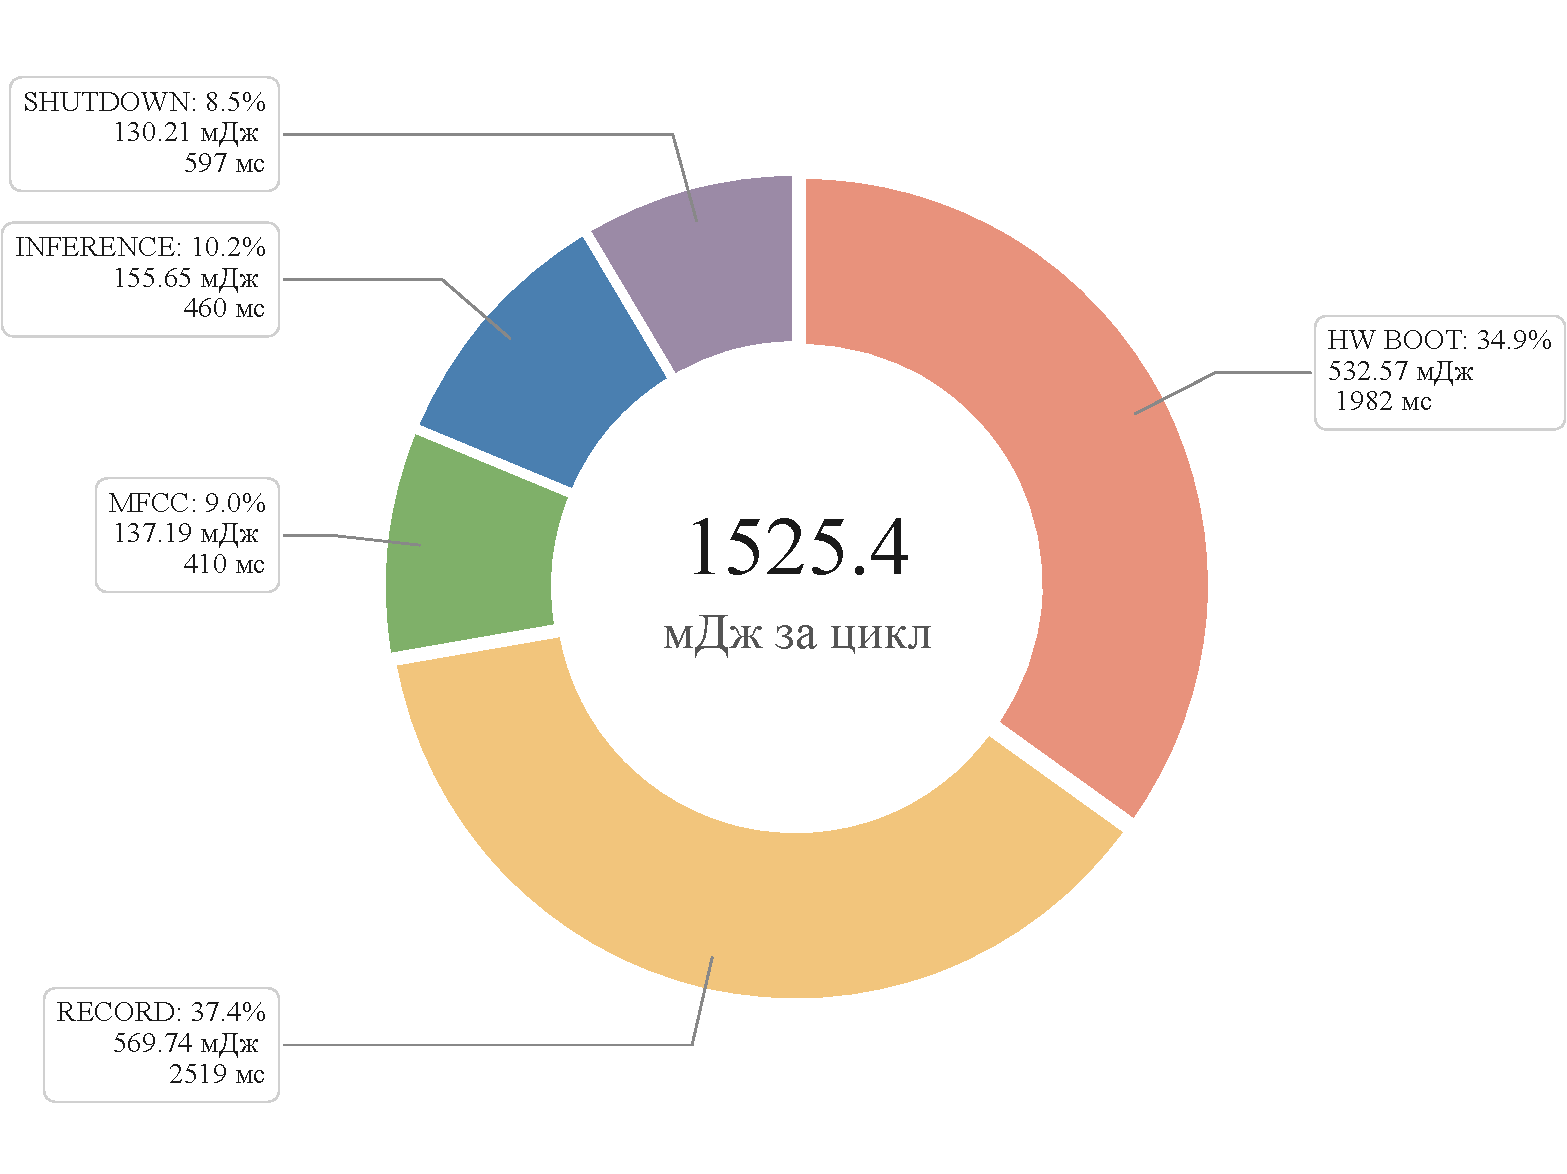
\includegraphics[width=0.85\textwidth]{assets/diagrams/fig4_7b_energy_donut_callouts.pdf}
	\caption{Распределение энергопотребления одного цикла каскадной обработки по этапам конечного автомата для выбранной модели $f104\_b5$ PTQ. Полная энергия цикла составляет 1525,4~мДж}
	\label{fig:energy_donut}
\end{figure}

Анализ декомпозиции приводит к ключевому выводу настоящей
работы. Собственно вычислительные этапы~--- извлечение
MFCC-признаков (9,0\%) и нейросетевой инференс (10,2\%)~--- в
сумме составляют 19,2\% общего энергобюджета цикла, тогда как
доминирующий вклад вносят \textit{сервисные} этапы:
аппаратная инициализация микроконтроллера после пробуждения
(34,9\%), захват аудио (37,4\%) и подготовка к переходу в
глубокий сон (8,5\%). Данное наблюдение качественно
согласуется с независимым выводом Cerutti и
др.~\cite{src:7} о доминирующем вкладе предобработки в общий
энергобюджет KWS-конвейера, однако дополняется следующей
особенностью каскадных архитектур: при переключении
микроконтроллера между режимами питания значимыми компонентами
энергобюджета становятся также инициализация подсистем после
пробуждения и подготовка к переходу в глубокий сон. Эти этапы
отсутствуют в традиционных конвейерах непрерывного мониторинга
и идентифицируются как самостоятельные значимые компоненты
энергобюджета именно в каскадных архитектурах с активным
управлением режимами питания.

\textit{Тем самым задача~5 введения выполнена.} Проведена
покомпонентная декомпозиция энергобюджета каскадного цикла,
выявившая доминирующий вклад сервисных этапов и определяющая
приоритетные направления дальнейшей оптимизации
(см.~подраздел~4.9).

\subsection{Сравнительная оценка автономности}

Согласно формуле~\eqref{eq:avg_power_v2} раздела~3, средняя
потребляемая мощность системы определяется энергией цикла и
частотой голосовых событий. Расчётное время автономной работы
от аккумулятора ёмкостью 2500~мА$\cdot$ч по
формуле~\eqref{eq:auto_time} рассчитано для трёх сценариев
эксплуатации, отличающихся частотой голосовых событий, и для
трёх вариантов аппаратной реализации, отличающихся током покоя
в режиме глубокого сна. Результаты приведены на
рис.~\ref{fig:battery_life}.

\begin{figure}[H]
	\centering
	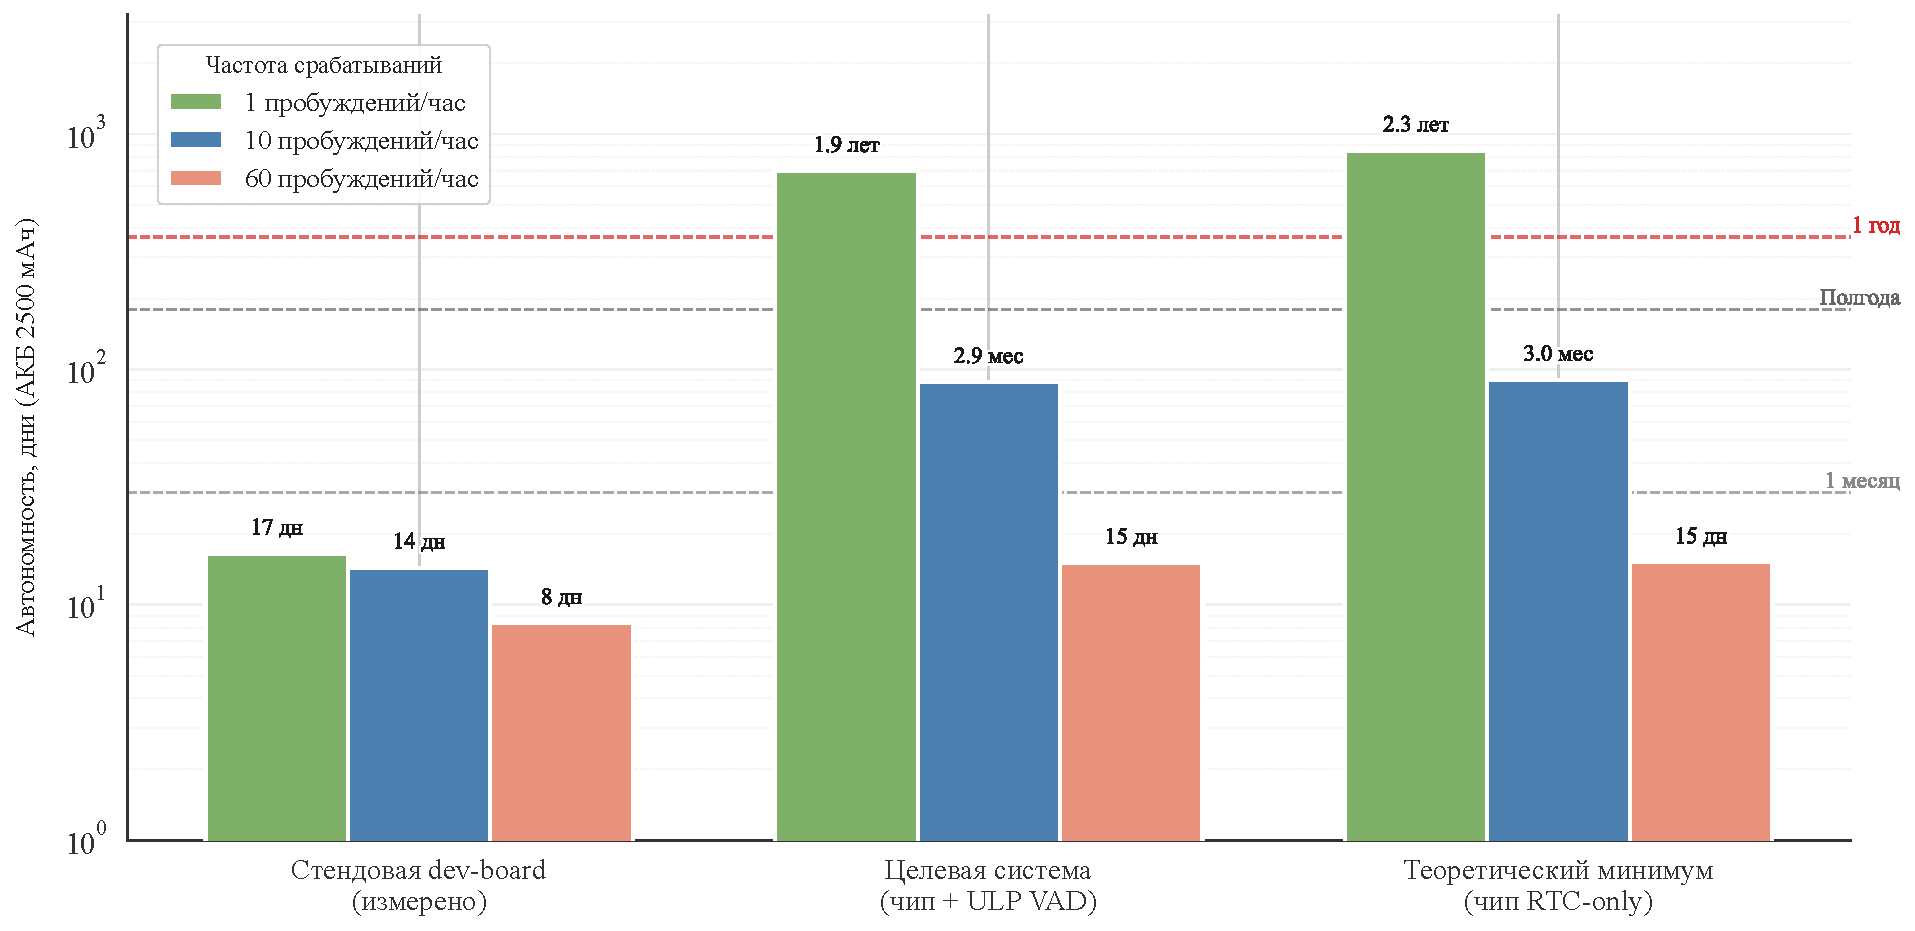
\includegraphics[width=1\textwidth]{assets/diagrams/fig4_X_battery_life.pdf}
	\caption{Расчётное время автономной работы системы от аккумулятора ёмкостью 2500~мА$\cdot$ч в зависимости от частоты голосовых событий для трёх вариантов аппаратной реализации}
	\label{fig:battery_life}
\end{figure}

Три варианта реализации соответствуют различным уровням
оптимизации аппаратной части системы при сохранении неизменной
каскадной архитектуры программного обеспечения.

\textit{Вариант~1~--- стендовая отладочная плата (измерено)}~---
текущая реализация на модуле ESP32-S3-Zero с обвязкой
отладочной платы, включающей линейный стабилизатор,
USB-UART-преобразователь, индикаторные светодиоды и
аналоговый модуль детектора звука LM393. Измеренный ток покоя
в режиме глубокого сна составляет 6,3~мА. Расчётная
автономность~--- от 8 до 17~суток в зависимости от частоты
срабатываний.

\textit{Вариант~2~--- целевая система с ULP VAD}~---
промышленная реализация с собственной печатной платой,
применением LDO ультранизкого тока покоя и заменой
аналогового компаратора на специализированный MEMS-сенсор с
интегрированной функцией пробуждения по звуку (wake-on-sound).
Расчётный ток покоя~--- порядка 30~мкА. Автономность увеличивается
до 15~суток при 60~пробуждениях в час, до 2,9~месяцев при
10~пробуждениях в час и до 1,9~лет при 1~пробуждении в час.

\textit{Вариант~3~--- теоретический минимум}~--- кристалл
ESP32-S3 в режиме deep sleep с активным RTC GPIO без
дополнительной обвязки. Согласно паспортным
характеристикам~\cite{src:9}, ток покоя составляет около
10~мкА. Автономность~--- 2,3~года при 1~пробуждении в час.

Сопоставление трёх вариантов показывает, что каскадная
архитектура программного обеспечения в сочетании с
оптимизацией аппаратной части позволяет достичь автономности
порядка лет при типичной частоте срабатываний бытового
устройства. Переход от отладочной платы к промышленной
реализации обеспечивает увеличение автономности более чем в
40~раз в режиме 1~пробуждение в час и сохраняет двукратное
преимущество даже при интенсивных 60~срабатываниях в час.
\textit{Тем самым подтверждено достижение цели ВКР} в части
снижения энергопотребления за счёт каскадного управления
режимами работы микроконтроллера: при ожидаемой частоте
голосовых событий типового бытового устройства предложенная
архитектура обеспечивает автономную работу длительностью от
недель до лет в зависимости от уровня аппаратной оптимизации.

\subsection{Дополнительные наблюдения и направления развития работы}

\subsubsection{Энергопотребление модуля в режиме глубокого сна}

Измеренное потребление модуля ESP32-S3-Zero в режиме глубокого
сна составило 6,3~мА, что превышает паспортное потребление
кристалла ESP32-S3 (7--8~мкА согласно технической документации
платформы~\cite{src:9}) примерно в 800~раз. Расхождение
объясняется суммой токов покоя компонентов обвязки модуля:
линейный стабилизатор напряжения, микросхемы флеш-памяти и
PSRAM в дежурном режиме, а также подключённый модуль детектора
звука LM393. Данное наблюдение представляет самостоятельное
инженерное значение: оно демонстрирует ценность измерений с
микроамперным разрешением на лабораторном стенде для
характеризации реального энергопотребления готового устройства
и подтверждает, что разрыв между паспортным потреблением
кристалла и фактическим потреблением серийного модуля не
является ограничением каскадной архитектуры как принципа, а
определяется обвязкой выбранной отладочной платы.

\subsubsection{Проекция на промышленную реализацию}

Декомпозиция энергобюджета настоящей работы выполнена на
отладочной плате со всеми присущими ей паразитными вкладами.
Покомпонентная проекция энергобюджета режима глубокого сна на
промышленную реализацию приведена в
табл.~\ref{tab:industrial_budget}.

% TODO: добавить microtypesetup
\begin{longtable}{|p{6.5cm}|c|}
	\caption{Покомпонентная проекция потребления в режиме глубокого сна для промышленной реализации}
	\label{tab:industrial_budget}                                                                        \\
	\hline
	\textbf{Компонент}                                                       & \textbf{Потребление, мкА} \\
	\hline
	\endfirsthead
	\hline
	\textbf{Компонент}                                                       & \textbf{Потребление, мкА} \\
	\hline
	\endhead
	\hline
	\endfoot
	ESP32-S3 в режиме глубокого сна с активным RTC IO~\cite{src:9}           & $\sim 10$                 \\ \hline
	LDO с ультранизким током покоя (HT7333, MCP1700 и подобные)              & $\sim 4$                  \\ \hline
	MEMS-микрофон с интегрированным wake-on-sound (Vesper VM1010 или аналог) & $\sim 10$                 \\ \hline
	Цифровой микрофон INMP441, обесточенный через MOSFET-ключ                & 0                         \\ \hline
	Подтягивающие резисторы, делители напряжения, паразитные токи            & $\sim 5$                  \\ \hline
	\textbf{Расчётное итоговое потребление в режиме ожидания}                & \textbf{$\sim 30$}        \\
	\hline
\end{longtable}


Расчётное потребление в режиме глубокого сна для промышленной
реализации лежит в диапазоне 30--70~мкА в зависимости от выбора
конкретных компонентов, что соответствует расчётной
автономности порядка нескольких месяцев при типичной частоте
срабатываний (см. рис.~\ref{fig:battery_life}, средний
столбец). Тем самым принципиальная достижимость заявленных во
введении показателей энергоэффективности подтверждена
покомпонентной декомпозицией, проведённой на основании
экспериментальных измерений.

\subsubsection{Направления дальнейшего развития}

Покомпонентная декомпозиция энергобюджета непосредственно
определяет приоритеты дальнейшего развития системы.

\textit{Уменьшение длительности этапа инициализации (HW BOOT,
	34,9\% энергобюджета цикла)}~--- наиболее значимое направление
оптимизации. Возможные подходы: перенос части инициализации в
RTC SRAM, сохраняющую содержимое при глубоком сне; применение
режима лёгкого сна вместо глубокого для уменьшения времени
повторной инициализации периферии; вынос инициализации
драйверов на сопроцессор ULP, способный работать параллельно
с пробуждением основного ядра.

\textit{Сокращение окна захвата аудио (RECORD, 37,4\%)}~---
применение скользящего кольцевого буфера, заполняемого
микрофоном в фоновом режиме при работе сопроцессора ULP,
позволит сократить активное окно захвата основным ядром с
2,5~секунд до фактической длительности произнесения команды.

\textit{Оптимизация обвязки модуля}~--- проектирование
собственной печатной платы с применением LDO с ультранизким
током покоя, замена аналогового VAD на специализированный
MEMS-сенсор с интегрированной функцией пробуждения по звуку
(wake-on-sound). Подобный подход реализован в академических
работах по сверхнизкопотребляющим аналоговым VAD~\cite{src:29,
	src:30}.

\textit{Дополнительная архитектурная оптимизация модели}~---
структурированное разрежение pointwise-свёрток, дистилляция
знаний из крупной модели в более компактную, что может дать
дополнительное снижение энергии нейросетевого инференса при
сохранении точности.

\textit{Верификация подхода на других платформах}~--- семейства
STM32U5 с механизмом LPBAM, nRF52840 с функцией wake-on-sound и
аналогичные платформы с поддержкой режимов глубокого сна и
внешнего пробуждения. Каскадная архитектура и методика
декомпозиции энергобюджета не привязаны к конкретной аппаратной
платформе.

\textit{Экспериментальное исследование стратегий
	постобработки}~--- агрегирование решений по скользящему окну,
применение корректора ложных отказов~\cite{src:28} для снижения
частоты ложных отказов без увеличения энергопотребления
модели.

\addtocontents{toc}{\protect\gdef\protect\cftsubsecnumwidth{2.1em}}
\subsection{Выводы по разделу}
\addtocontents{toc}{\protect\gdef\protect\cftsubsecnumwidth{1.55em}}

В настоящем разделе представлены результаты экспериментальной
апробации предложенной каскадной KWS-системы на платформе
ESP32-S3 и их интерпретация в терминах задач, поставленных во
введении. Получены следующие основные результаты.

\begin{enumerate}
	\item Систематическое исследование 134~архитектур DS-CNN в
	      пространстве гиперпараметров (filters $\times$ blocks)
	      выявило плато точности при $F \geq 80$, $B \geq 4$ в
	      пределах статистической погрешности оценки.
	      Построенная Парето-граница в координатах
	      <<точность~$\times$~размер модели>>
	      (рис.~\ref{fig:pareto_size_acc}) показала, что
	      эталонная конфигурация Hello Edge DS-CNN-M не является
	      Парето-оптимальной для исследованной задачи на
	      платформе ESP32-S3.

	\item Сравнение методов квантизации PTQ и QAT, проведённое
	      на двух уровнях обобщения (детально на 4~архитектурах и
	      агрегированно на 63~парах), показало, что для
	      разрядности INT8 98\% парных различий между методами
	      укладываются в коридор статистической погрешности
	      $\pm 0{,}65$~п.п. при медиане $+0{,}048$~п.п. Метод PTQ
	      является предпочтительным как обеспечивающий
	      сопоставимую точность при существенно меньшей
	      вычислительной стоимости. \textit{Задача~3 введения
		      выполнена.}

	\item Послойная декомпозиция времени инференса на ESP32-S3
	      выявила доминирующий вклад pointwise-свёрток
	      (50--86\% времени инференса в зависимости от размера
	      модели) с сверхлинейной зависимостью от числа
	      фильтров, что определяет приоритеты архитектурной
	      оптимизации.

	\item По Парето-критерию <<точность~$\times$~энергия
	      инференса>> выбрана финальная модель \texttt{f104\_b5}
	      PTQ (96,12\% точности, 101~КБ размер, 149,6~мДж/инференс),
	      обеспечивающая компромисс между точностью, размером и
	      энергопотреблением и превосходящая эталонную
	      Hello~Edge конфигурацию по совокупности критериев.

	\item Качество классификации выбранной модели
	      охарактеризовано по совокупности метрик precision,
	      recall, F1-score по каждому классу
	      (табл.~\ref{tab:classification_metrics}); macro avg
	      F1 = 0,9432, weighted avg F1 = 0,9580. Структура
	      ошибок концентрируется на парах акустически близких
	      слов и сохраняется при квантизации, что подтверждает
	      корректность процедуры квантизации.

	\item Выполнена покомпонентная декомпозиция энергобюджета
	      каскадного цикла. Установлено, что собственно
	      вычислительные этапы составляют 19,2\% энергобюджета,
	      тогда как доминирующими являются сервисные этапы
	      (инициализация 34,9\%, захват аудио 37,4\%,
	      завершение 8,5\%). Идентификация инициализации и
	      завершения как самостоятельных значимых компонентов
	      энергобюджета, не учитываемых в моделях непрерывного
	      мониторинга, составляет содержание главного
	      исследовательского результата работы.
	      \textit{Задача~5 введения выполнена.}

	\item Сравнительная оценка показала, что предложенная
	      каскадная архитектура программного обеспечения в
	      сочетании с переходом от отладочной платы к
	      промышленной аппаратной реализации обеспечивает
	      увеличение расчётного времени автономной работы от
	      8--17~суток до 2,9~месяцев~--- 1,9~года в зависимости
	      от частоты голосовых событий, что подтверждает
	      достижение цели работы в части снижения
	      энергопотребления за счёт каскадного управления
	      режимами работы микроконтроллера.

	\item Определены приоритетные направления дальнейшего
	      развития системы: уменьшение длительности этапа
	      инициализации, использование скользящего кольцевого
	      буфера на сопроцессоре ULP для сокращения окна
	      захвата аудио, оптимизация обвязки модуля с
	      применением LDO ультранизкого тока покоя, замена
	      аналогового VAD на специализированный MEMS-сенсор,
	      верификация подхода на других микроконтроллерных
	      платформах.
\end{enumerate}
